\chapter{Analysing the signals}
\label{ch:roundb}

\begin{instructions}
Author update, 8 Nov: include both MJu26a trains as case-study candidates---the long CH15 train at 206--283\,h and
the four-hour CH14 excerpt. The accepted-catalogue reconciliation supplies 143 and 32 separately anchored
downward excursions, respectively, with machine-proposed extents and explicit train-level acceptance. Inspect
and finalise boundaries before using their durations as event measurements. Show each train in the signal,
then an enlarged example, shape overlays and the timing/spacing of its individual members. Distinguish the
existing individual judgements from the author's later train-level inclusion; do not count the old five-channel
copy, excerpt and full MJu26a recording as independent data. Sources and the proposed analysis are in
\src{docs/thesis/data/accepted_catalogue/REPORT.md}. This follow-up does not change the historical g-11 results
or imply propagation, a physiological oscillator, or a complete low-amplitude event census.
\end{instructions}

\begin{instructions}
About 7--9 pages: ten short studies (B4 is being redesigned separately), each about half a page plus one figure.
The list was fixed on 27 Oct (Round 4) and B3's design on 28 Oct (Round 5). B4's page was specified in the
cross-channel workshop (27 Oct) but is not yet built. Experiments freeze Tue 3 Nov.

Every study states these decisions:
\begin{itemize}
  \item \textbf{Historical grouping}: g-11, one representative per de-duplicated event in the 5 November snapshot
        (Section~\ref{sec:families}). The reported family tests below retain that population. The later accepted
        inventory is a collection of observations, including sequence parents; it is not automatically a new
        morphology grouping or an exhaustive timing census.
  \item \textbf{Counts are of events, not members} (the events table). The rule: collapse twins ($\ge$90\,\% mutual
        overlap); keep a container with its parts; join units at $\ge$50\,\% overlap or gaps $\le$3\,s, never through a
        container. Joining on any overlap made one 93-minute train a single 111-part event.
  \item \textbf{Datasets}: M2\_aug and M2\_concat (both oyster, 1\,Hz); CO\_fs2 (chocolate oyster) and
        LM\_fs2 (lion's mane); and the 2\,Hz copies of
        MJu26a, SH and SO (27 Oct). Excluded:
        \begin{itemize}
          \item MJu26a's five-channel copy (CH10, 13--16);
          \item M4, the exam;
          \item every other copy of a recording at another rate.
        \end{itemize}
  \item \textbf{On the site}: each question is answered on the site's own pages and templates. Backend or cluster
        computation is allowed where a page cannot do the arithmetic.
\end{itemize}
Candidate notes and evidence: \src{docs/rq_roundB/README.md} and \src{docs/rq_roundB/notes/drop-motif-sequences.md}.
\end{instructions}

The three research questions asked what the instrument can do. This chapter uses it to ask what the signals do: a set of shorter questions about sequences, recovery, shapes, channels, detectors, time scales and methods borrowed from other fields. Each is answered with the site as it stood, and each is judged against a null.

\section{How the questions were chosen}

\begin{instructions}
Rules: answerable on the site with little new building; one null per question; one figure; a stated claim and a
stated non-claim. Table~\ref{tab:roundb} is the list as fixed on 27 Oct. ``Small'' builds are the two approved in
Round 4: the Intervals nulls and the sequence morph readout.

B3 as fixed also asked whether an excitable-system model describes the drop cycles beyond noise. That half is parked
(4 Nov, Section~\ref{sec:rb_models}), so the table lists only the restitution question.
\end{instructions}

\begin{table}[htbp]
\caption{The questions studied in this chapter: the site page that answers each, its data, its null, and the building it needed. B7 (multiscale entropy) and B8 (motif prevalence) were not run; they are future work (Section~\ref{sec:futurework}).}
\label{tab:roundb}
\footnotesize
\begin{tabularx}{\textwidth}{@{}l >{\raggedright\arraybackslash}X >{\raggedright\arraybackslash}p{3.1cm} >{\raggedright\arraybackslash}p{2.5cm} >{\raggedright\arraybackslash}p{2.3cm} >{\raggedright\arraybackslash}p{1.5cm}@{}}
\toprule
\textbf{\#} & \textbf{Question} & \textbf{On the site} & \textbf{Data} & \textbf{Null} & \textbf{Build}\\
\midrule
B1 & Are the intervals between events regular, bursty or random? & Interrogation $\rightarrow$ Intervals (LV, CV2) & drop-detector events, active sets & random timing; shuffled intervals & small\\
B2 & Do drop sequences change shape step by step more than chance? & Library $\rightarrow$ Sequences, on g-11 & M2\_aug, M2\_concat, CO, LM & shuffled order & small\\
B3 & Does a drop's recovery depend on the gap before it? & Event shape and Intervals (restitution) & sequences and chains; the drop-detector census & shuffled gaps & backend\\
B4 & Is cross-channel activity propagation or a shared-ground artefact? (plan RQ6) & Explore $\rightarrow$ Cross-channel (the explorer, S0--S1 at least) & the seven sets & rotation; random time & explorer build\\
B5 & What do the Discovery Maps show about when and where detectors fire? & Discovery $\rightarrow$ Map & all swept sets & paired surrogate runs; time-shifted rates & none\\
B6 & Do the same shape families occur across recordings and species? & Library $\rightarrow$ Atlas, Recurrence, on g-11 & M2\_aug, M2\_concat, CO, LM & shuffled recording labels & none\\
B9 & Do event durations cluster at preferred scales? & \texttt{cwt\_events} & all swept sets & AAFT surrogates & none\\
B10 & At which time scales does structure beyond noise appear? & \texttt{motif\_lengths}; CNN templates at 1, 10, 60\,min; \texttt{spike\_event\_\allowbreak features} & M2\_aug, M2\_concat, CO, LM, MJu26a & AAFT surrogates & none\\
B11 & Do the detectors find the same events on the newer datasets? & Discovery $\rightarrow$ Compare; Compare every stage & CO, LM, MJu26a, SH, SO & per-run surrogate & none\\
B12 & Do spike and drop shapes and intervals differ between recordings and species? & Interrogation $\rightarrow$ Event shape, Intervals, on accepted events & M2\_aug, M2\_concat, CO, LM & shuffled recording labels & none\\
\bottomrule
\end{tabularx}
\end{table}

\subsection{What the expanded Library changes}

The completed follow-up reviews enlarged the accepted inventory to 2,718 spans across eight recordings. This supplies more material for the questions in this chapter, particularly the inclusion of MJu26a in the Library family comparisons and accepted examples from shiitake and snow oyster. MJu26a was already represented by its five-channel copy in the earlier blind shape comparison; its additional channels therefore broaden that recording's coverage. The family-composition tests used g-11, while the shape comparisons used the 716 accepted blind detector-review spans. Those results retain their original denominators until equivalent analyses are repeated on the expanded material.

The main distinction is between collecting examples and observing a sequence. A diverse sample of accepted shapes can strengthen a waveform comparison, but the gaps between sampled examples cannot describe the timing of all events in a recording. A broad accepted span can also contain several events. Individual waveforms must remain separate entries, with a train or sequence linking them in order; shared recovery context is insufficient reason to merge them. The CH14 case below applies this distinction explicitly. For B1--B3, checked identities and onset/recovery boundaries are more valuable than simply adding further isolated interesting windows. For B6 and the shape part of B12, the enlarged material needs regrouping and source-aware comparisons, with individual trains prevented from dominating the apparent species differences.

The machine-only questions have a different dependency. The recovered classical detectors can already extend selected comparisons, while a complete new detector-agreement census for B5 and B11 still requires the remaining CNN tasks. Their completion is not required to review the available classical proposals. A further blind queue therefore prioritises SH and SO, other MJu26a channels and periods, and a range of amplitudes, durations and provisional polarities. It also includes background controls and the planned repeat checks. Those labels are intended to broaden the collection and assess judgement consistency; their selected composition does not supply an unbiased estimate of event prevalence.

\section{A longer reviewed train on MJu26a CH14}
\label{sec:mjuch14train}

\subsection{The selection and its individual events}

A further review examined a selected train on MJu26a CH14 from 382.5 to 473.2 hours, a span of approximately 90.7 hours (Figure~\ref{fig:mjuch14train}). This is a longer part of the same physical channel containing the earlier four-hour excerpt. It is distinct from the CH15 train at 206--283 hours. BEADS preprocessing, with a 2,000\,s baseline period and downward polarity, was followed by a signal threshold at $-0.957$\,mV, a minimum duration of 1.5\,s and short context margins. The resulting candidates were reviewed by the researcher, yielding accepted observations linked to 509 spans in the reconciled catalogue.

The trace shows repeated downward excursions alongside a substantial change in the baseline over the longer recording. At a closer scale, neighbouring deflections differ in depth, recovery and internal structure. The accepted detector intervals often capture only the narrowest part of a drop, while some small deflections occur during the recovery of a larger one. Thus 509 accepted spans should not be interpreted as 509 final, independently bounded spikes. The four-hour excerpt and the L\_LM and 2\,Hz copies are linked to their parent coordinates, rather than added as further independent recordings.

An exploratory separation pass used the 10\,Hz parent signal, smoothed with a Gaussian standard deviation of 0.5\,s, and located negative extrema with at least 1\,mV prominence and 3\,s separation. Each of the 534 positive source observations was linked to the extrema it contained. A cropped observation could be linked to a nearby extremum only where its prominence-width interval covered at least half the observed span and the extremum was no further away than the shorter of 120\,s or the observed span's duration. Distinct extrema retained distinct identities even where their recovery windows overlapped. This produced 530 individual event proposals supported by the positive observations. Thirteen observations contained several retained extrema; 19 could not be mapped cleanly and remain unresolved. The parent observations and their ordered child proposals are preserved separately. These numbers describe the extraction rule, rather than 530 new independent human judgements.

\begin{figure}[htbp]
\centering
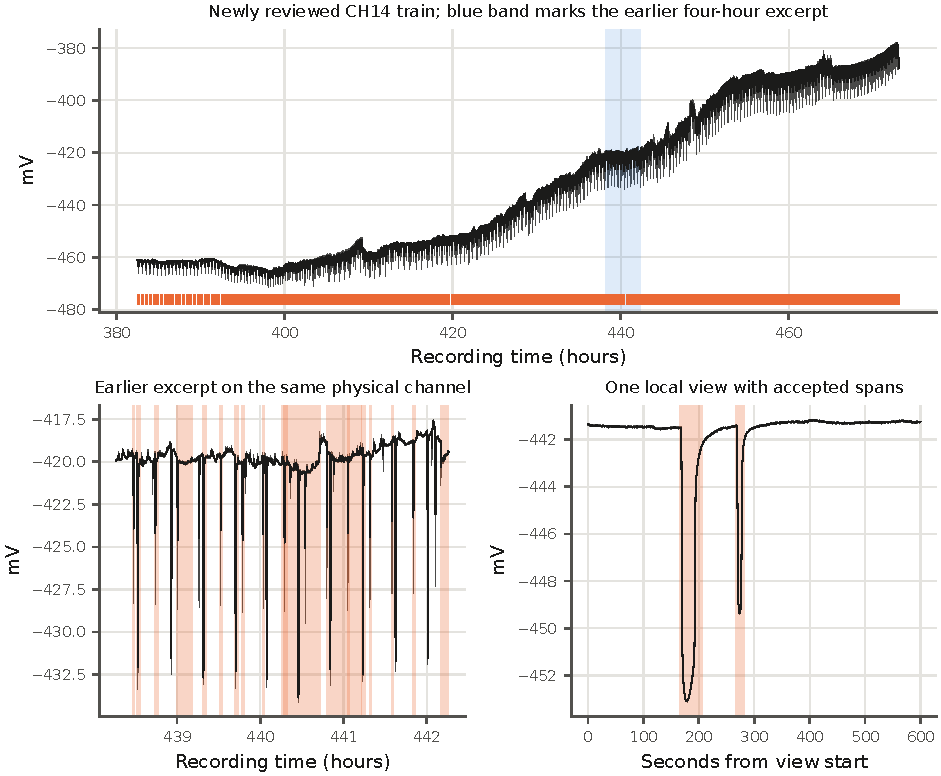
\includegraphics[width=\textwidth]{new/ch10_mju_ch14_reviewed_train.pdf}
\caption{The newly reviewed MJu26a CH14 train and its relation to the earlier four-hour case study. Top: the approximately 90.7-hour signal, displayed as a minimum--maximum envelope to preserve narrow excursions; orange ticks mark accepted-span starts and the blue band locates the older excerpt. Bottom left: that four-hour region drawn from the same 10\,Hz parent channel, with accepted spans shaded orange. Bottom right: a local view around 427 hours showing a deep drop, its recovery and a following smaller drop. Shading marks the accepted spans, rather than asserting completed onset-to-recovery boundaries. The panels show different time and voltage scales. The repeated shapes and baseline drift are descriptive features of this selected recording; the plot does not establish a physiological oscillator or propagation between channels.}
\label{fig:mjuch14train}
\end{figure}

\begin{figure}[htbp]
\centering
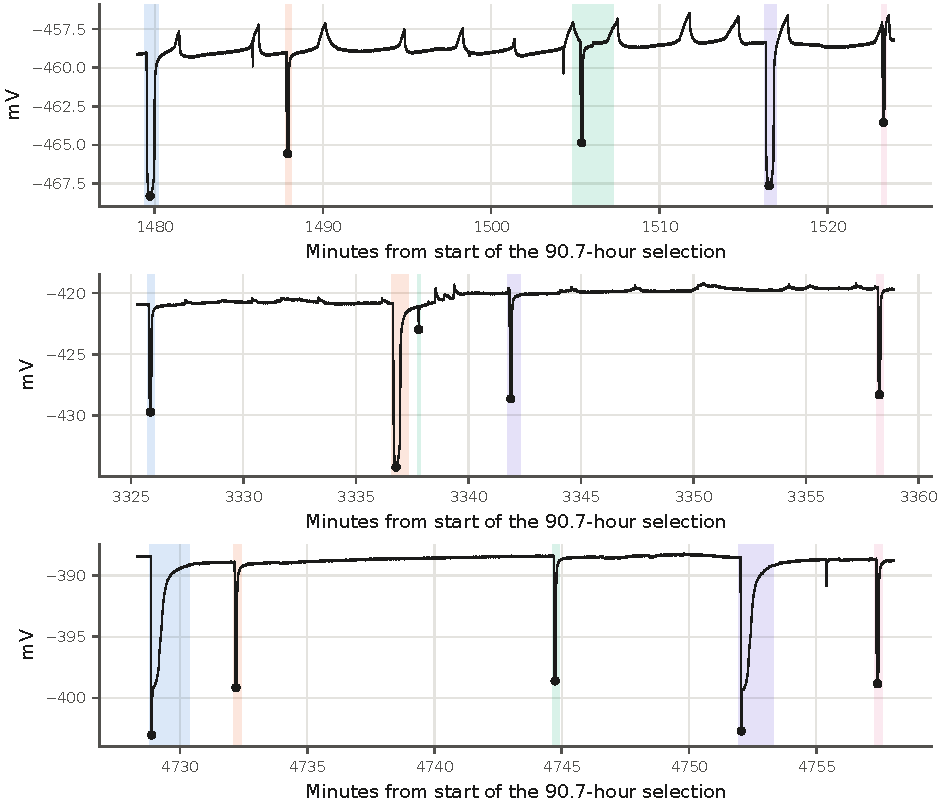
\includegraphics[width=\textwidth]{new/ch10_ch14_separate_events.pdf}
\caption{Separating individual events within the longer CH14 train. The panels show five consecutive supported proposals near the middle of each event-order third, with the surrounding signal retained. Black dots locate the individual trough anchors. Different colours distinguish neighbouring proposed extents and do not denote different waveform families. An uncoloured deflection is outside the five displayed proposals and is not thereby labelled uninteresting. Recovery is bounded by the next detected excursion, so a following event remains a separate member rather than being absorbed into the preceding event's tail. The onsets and recovery extents are machine proposals linked to the earlier accepted observations, and remain available for explicit boundary checking.}
\label{fig:ch14individuals}
\end{figure}

\subsection{Variation in amplitude and recovery}

The individual proposals show that the train cannot be described adequately by one average waveform. Onset-to-trough depth had a median of 9.22\,mV, with a 5th--95th percentile range of 2.47--14.65\,mV. The median depth increased from 6.57\,mV in the first event-order third to 9.13\,mV in the middle third and 10.08\,mV in the last. Several depth tracks are visible later in the recording (Figure~\ref{fig:ch14measures}), alongside smaller intervening deflections. These are within-recording changes; they are not sufficient evidence of distinct physiological event types.

The event-shape routines measured each proposal on the native signal, using the proposed onset and trough anchors. Onsets used the existing steepest-fall shoulder rule, bounded after the preceding extremum. Half recovery means the first return from the trough through half of the onset-to-trough depth. It was measurable for 529 of the 530 proposals, with a median of 2.49\,s and a 5th--95th percentile range of 0.83--17.44\,s. A return through half the depth is different from a complete recovery: 25 proposals did not reach the 95\,\% recovery level before the next detected excursion. Their extents were censored there, preserving the next event's separate identity. These proposal-based measurements should therefore be checked before being used as final duration statistics or evidence for restitution.

\begin{figure}[htbp]
\centering
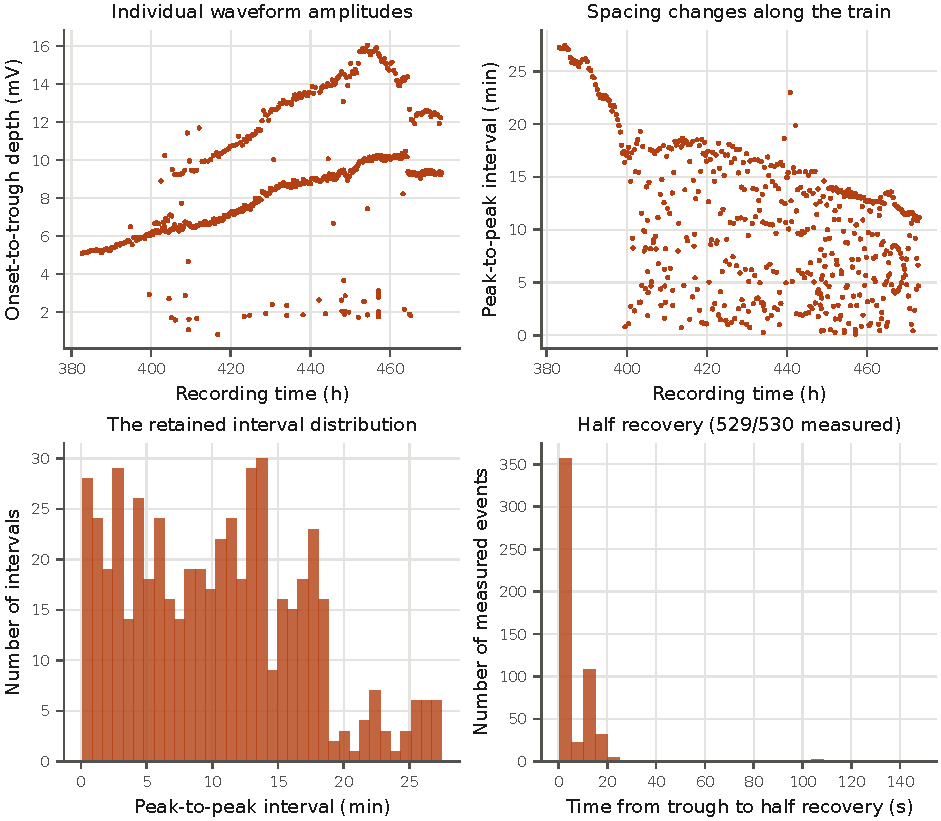
\includegraphics[width=\textwidth]{new/ch10_ch14_event_measures.pdf}
\caption{Exploratory measurements of the 530 individually anchored CH14 proposals supported by positive review observations. Top left: onset-to-trough depth against recording time, showing changing depths and several later tracks. Top right: the interval from each retained trough to the preceding retained trough, plotted at the later event's time. Bottom left: the distribution of these 529 intervals. Bottom right: the 529 measurable trough-to-half-recovery times; one proposal did not reach that level within its permitted recovery search. Amplitudes and recovery values use the native signal with machine-proposed anatomy. Half recovery is not full event duration. The retained events are a selected, reviewed subset, and the plots do not establish a complete census of every smaller fluctuation in the train.}
\label{fig:ch14measures}
\end{figure}

\subsection{Timing structure and sensitivity to event definition}

The median interval between retained troughs was 603\,s, or approximately 10.0 minutes, with a 5th--95th percentile range of 51--1,359\,s. These are peak-to-peak intervals, which depend less on the unfinished onset boundaries. Their local variation was 0.708 and CV2 was 0.785. Both were below the 95\,\% bands from 1,000 random-timing draws with the same number of points and observed time span: LV 0.905--1.093 and CV2 0.943--1.060. The retained train was therefore more regular locally than this homogeneous random-timing reference, rather than perfectly periodic.

Shuffling the retained intervals gave an LV band of 0.724--0.811, also above the observed value (two-sided permutation $p=0.006$). Under the 1\,mV rule, neighbouring gaps were therefore more alike than the same gaps in random order. This part of the result depended on which smaller events were included (Table~\ref{tab:ch14sensitivity}). Increasing the prominence floor to 2\,mV retained 503 supported extrema and preserved the difference from random timing, but the gap-order result disappeared. The observed structure therefore supports a selected, relatively regular train, while its finer serial organisation depends on the operational event definition.

\begin{table}[htbp]
\centering\small
\caption{Sensitivity of the selected CH14 train to the prominence floor, with 0.5\,s smoothing and 3\,s minimum separation held fixed. Counts include only extrema linked to positive review observations. The nulls use 1,000 draws and the existing two-sided permutation calculation. These are exploratory comparisons on a visually selected train, rather than a new recording-wide discovery test.}
\label{tab:ch14sensitivity}
\begin{tabular}{@{}rrrrr@{}}
\toprule
\makecell[r]{\textbf{Prominence}\\\textbf{floor (mV)}} & \makecell[r]{\textbf{Supported}\\\textbf{extrema}} & \textbf{LV} & \makecell[r]{\textbf{Random timing}\\\boldmath$p$} & \makecell[r]{\textbf{Shuffled gaps}\\\boldmath$p$}\\
\midrule
0.5 & 542 & 0.712 & 0.002 & 0.002\\
1.0 & 530 & 0.708 & 0.002 & 0.006\\
2.0 & 503 & 0.682 & 0.002 & 0.885\\
\bottomrule
\end{tabular}
\end{table}

This case complements the full-channel detector census below. A deliberately selected, human-accepted train can show regularity even where the broader census did not establish recording-wide regularity after correction. The two tests use different selections and counting units. Likewise, the observed amplitude changes do not establish a mechanism, and a single-channel train cannot establish propagation between channels. The main contribution is a traceable progression from reviewed spans to individual waveform proposals and ordered sequence structure, with the unresolved observations, recovery censoring and threshold sensitivity retained explicitly.

% Completed queue 45 / run 8750; frozen review snapshot and canonical spans in
% data/reviews_completed_20261108/. Native CH14 data, no duplicate-copy counts.
% Individual-event follow-up: data/event_hierarchy_20261108/ch14_case.json and
% ch14_individual_proposals.csv; reviewed_event_hierarchy.py. No new human labels.

\section{Sequences and timing}
\label{sec:rb_sequences}

\begin{instructions}
\textbf{B1}, intervals:
\begin{itemize}
  \item Measure: LV \cite{shinomoto2003lv} and CV2 \cite{holt1996cv2} of event onsets, per channel.
  \item Nulls: a rate-matched Poisson train (LV $=1$), and the same intervals shuffled.
  \item Data: drop-detector events on the active sets, and the \texttt{chain\_cycles} chains.
  \item Build: done 28 Oct. The Intervals block reports both nulls, 1,000 seeded draws per group
        (\src{Working/interrogation/intervals.py}).
  \item First read (M2\_aug, \texttt{drop\_detection\_v1}, one 721\,h run per channel):
        \begin{itemize}
          \item against random timing, LV and CV2 sit inside the band on most channels. CH3 ($n=127$) is more regular:
                LV 0.72 against 0.82--1.20, $p=0.004$, which is borderline once 16 channels are corrected for;
          \item against shuffled gaps, LV sits below the band on 11 of 16 channels. Neighbouring gaps are more alike
                than their mix implies: the rate drifts slowly over the 30 days.
        \end{itemize}
  \item \textbf{Final read (5 Nov)}, on every recording with a complete \texttt{drop\_detection\_v1} run: 56 channels
        of M2\_aug, M2\_concat, CO, LM and MJu26a (its 2\,Hz copy, imported 5 Nov; it replaces MJu26a's five-channel copy,
        CH10, 13--16). SH and SO have no \texttt{drop\_detection\_v1} run yet. Each channel is one complete run, the same
        kind as B12's. 44 channels have the three events a measure needs. Benjamini--Hochberg at 0.05 runs across
        those 44, separately for each measure and null. Sources: \src{scripts/thesis/b1_intervals.py},
        \src{docs/rq_roundA_2/findings/b1-intervals-2026-11-05.md}; ledger J1b; Figure~\ref{fig:b1lv}.
        \begin{itemize}
          \item \textbf{Against random timing, random-like.} LV is outside the Poisson band at $p<0.05$ on 9 of 44
                channels, but none survives correction. CV2 leaves two channels more regular than random: M2\_aug CH3
                (127 events, CV2 0.78) and LM CH1 (30 events, LV 0.47, CV2 0.60).
          \item \textbf{Against shuffled gaps, neighbouring gaps are more alike than their mix} on 18 of 44 channels
                after correction (LV), on every recording: M2\_aug 9 of 16, M2\_concat 2 of 15, LM 2 of 4, CO 1 of 2,
                MJu26a 4 of 7. The rate drifts slowly. One M2\_concat channel (CH6) goes the other way: long and short
                gaps alternate.
          \item \textbf{Caveat.} 20 channels have fewer than 10 events, among them nine of MJu26a's 16 (at most two
                events each at 2\,Hz) and most of CO's. The read rests on the busier channels.
        \end{itemize}
\end{itemize}

\textbf{B2}, sequence morph:
\begin{itemize}
  \item Measure: along each drop sequence, the fraction of steps smaller than the end-to-end change.
  \item Null: the same events in shuffled order.
  \item Data: the Library's sequences. Of the 118 on 28 Oct, 99 sit on inactive recordings (98 on F2A). g-11 is the
        final grouping, so the sequences are read as they stand.
  \item Build: done 28 Oct (\src{Working/library/morph.py}). Library $\rightarrow$ Sequences and the Atlas show it.
  \item First read of the morph fraction: 0 of 5 testable sequences beat their shuffle, against 0.2 expected by chance.
        The fraction is coarse. A shuffled order also scores 1 whenever its two ends lie far apart, so even a perfect
        morph cannot reach $p<0.05$ below about 20 elements.
  \item The step-size companion (added 28 Oct, at the researcher's choice): the mean shape distance between
        neighbouring events, against the same shuffled orders. It can judge sequences of five or more elements. It asks
        a weaker question than the morph fraction: a steady morph passes it, but so do runs of near-identical events,
        and it does not tell the two apart (a test pins this). Sequences built from label chains can pass it by
        construction. Both p values per sequence come from the same orders, so they are not independent evidence.
  \item First read of the step size (headless, full-resolution samples): 5 of the 19 sequences on active recordings
        have neighbours more alike than shuffled at $p<0.05$, against 0.9 expected by chance; 4 survive
        Benjamini--Hochberg. Their step ratios are 0.58--0.84. Two of them are long enough for the morph fraction too
        (sq-1, 67 events; sq-4, 26): their steps are smaller than shuffled ($p=0.001$, 0.010) but their fraction is
        not higher. That points to persistence rather than a steady morph.
  \item Five other sequences go the other way (ratios 1.15--1.33, $p>0.97$): neighbours are less alike than random
        pairs. Four of them alternate visibly in stretches, one family every other element (F-80 in three, F-66 in one). That
        direction was not the question asked, so report it as an observation only.
\end{itemize}
\end{instructions}

\begin{figure}[htbp]
\centering
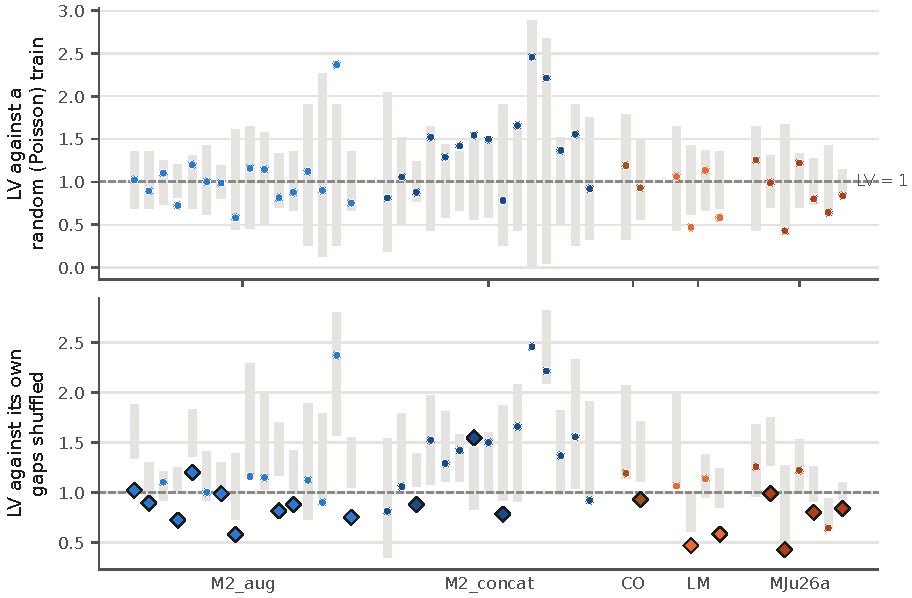
\includegraphics[width=\textwidth]{new/ch10_b1_lv.pdf}
\caption{B1: the LV of the intervals between \texttt{drop\_detection\_v1} events, one point per channel, coloured by recording. Grey bars are each null's 95\,\% band: a rate-matched random (Poisson) train (top) and the channel's own gaps shuffled (bottom). Diamonds pass Benjamini--Hochberg across the 44 measurable channels. No channel leaves the random band, but on 18 channels neighbouring gaps are more alike than shuffled: the timing is random-like with a drifting rate.}
\label{fig:b1lv}
\end{figure}

\begin{figure}[htbp]
\centering
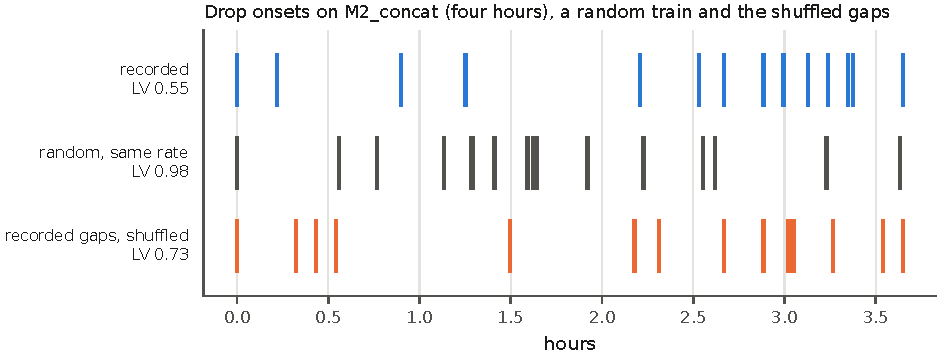
\includegraphics[width=\textwidth]{new/ch10_b1_train.pdf}
\caption{B1 in the signal: the drop onsets of four hours of M2\_concat (top; the train of Figure~\ref{fig:anatomytrain}), a random (Poisson) train with the same number of onsets over the same time (middle), and the recorded gaps in a shuffled order (bottom), each with its LV. Neighbouring gaps in the recorded train are more alike than in the shuffled order (LV 0.55 against 0.73): short gaps follow short ones and long follow long, which is what a slowly drifting rate looks like.}
\label{fig:b1train}
\end{figure}

\section{Recovery and the gap before it}
\label{sec:rb_models}

\begin{instructions}
\textbf{B3}: does a drop's recovery depend on the gap before it? Only the restitution test is reported here.

The model half is parked, at the researcher's decision (4 Nov). That covers FitzHugh--Nagumo, Izhikevich and the
fall-plus-recovery kernel judged by held-out cycles, and the 4 Nov follow-up on the longest trains with van der Pol,
Morris--Lecar and phase response curves.
\begin{itemize}
  \item \textbf{Why:} the models fit the drop cycles, but they fit fake cycles cut from noise about as well, so the fits
        say nothing specific about fungal signals.
  \item \textbf{Where it is:} the parked text and figures are in \src{docs/thesis/parked/ch10_b3_models.tex}.
  \item \textbf{Its findings:} \src{docs/rq_roundA_2/findings/fhn-fit-2026-10-26.md}, the model half of
        \src{docs/rq_roundA_2/findings/b3-restitution-tracking-2026-10-28.md}, and
        \src{docs/rq_roundA_2/findings/b3-long-trains-2026-11-03.md}.
  \item \textbf{If modelling is discussed:} only in general terms, in Chapter~\ref{ch:discussion}.
\end{itemize}

\textbf{The restitution test} comes from cardiac electrophysiology. Does a drop's recovery shorten when the gap before
it was short? It needs no model fit.
\begin{itemize}
  \item \textbf{Measures:} recovery times come from Event shape and gaps from Intervals.
  \item \textbf{Null:} the gaps are shuffled within each sequence.
  \item \textbf{Data:} primarily trains (the Library's sequences and the \texttt{chain\_cycles} chains); secondarily,
        consecutive events in the drop-detector census.
  \item \textbf{Code:} \src{Pipelines/fhn/run_b3.py}.
\end{itemize}
\end{instructions}

\begin{instructions}
Results (28 Oct). Sources: \src{docs/rq_roundA_2/findings/b3-restitution-tracking-2026-10-28.md}; ledger J3;
Figure~\ref{fig:b3restitution}. The method:
\begin{itemize}
  \item recovery is Event shape's half-recovery time, measured on the raw channel samples;
  \item the gap is onset to onset;
  \item each train gets 1,000 permutations of its own gaps;
  \item trains are combined by a $\sqrt{n}$-weighted signed Stouffer $z$.
\end{itemize}
The results:
\begin{itemize}
  \item \textbf{Within trains, no restitution.} Over 74 scorable sequences (987 pairs), the raw lean ($z=+2.9$)
        vanishes given depth ($+0.6$) or event order ($+0.7$). The same correlation with the gap \emph{after} each
        drop is larger ($+9.9$): recovery is cut off at the next drop, which is a censoring artefact. The three long
        chains agree.
  \item \textbf{Across census gaps, a modest relation on the two M2 recordings.} Across the drop-detector census's
        hours-long gaps, both show a restitution-like relation: M2\_aug $z=+5.0$ and M2\_concat $+3.1$, both oyster (pair-weighted
        $\rho\approx0.25$). It survives depth, order and the next gap, and is halved by the fall's duration. LM and
        CO are not significant (3 and 2 channels).
  \item \textbf{Not scored.} 43 of the 117 sequences, mostly reishi: 339 of 1,298 reishi events never recover halfway
        before the next drop.
\end{itemize}

What it can claim:
\begin{itemize}
  \item no within-train restitution;
  \item a modest restitution-like relation across census gaps on M2\_aug and M2\_concat (both oyster).
\end{itemize}
What it cannot claim: any mechanism for the census relation.

Caveat: the Library's stored recovery times are measured on detrended snippets, so they differ from these by design.
Open follow-up: a censoring-aware recovery, by survival analysis with the next onset as the censoring time.
\end{instructions}

\begin{figure}[htbp]
\centering
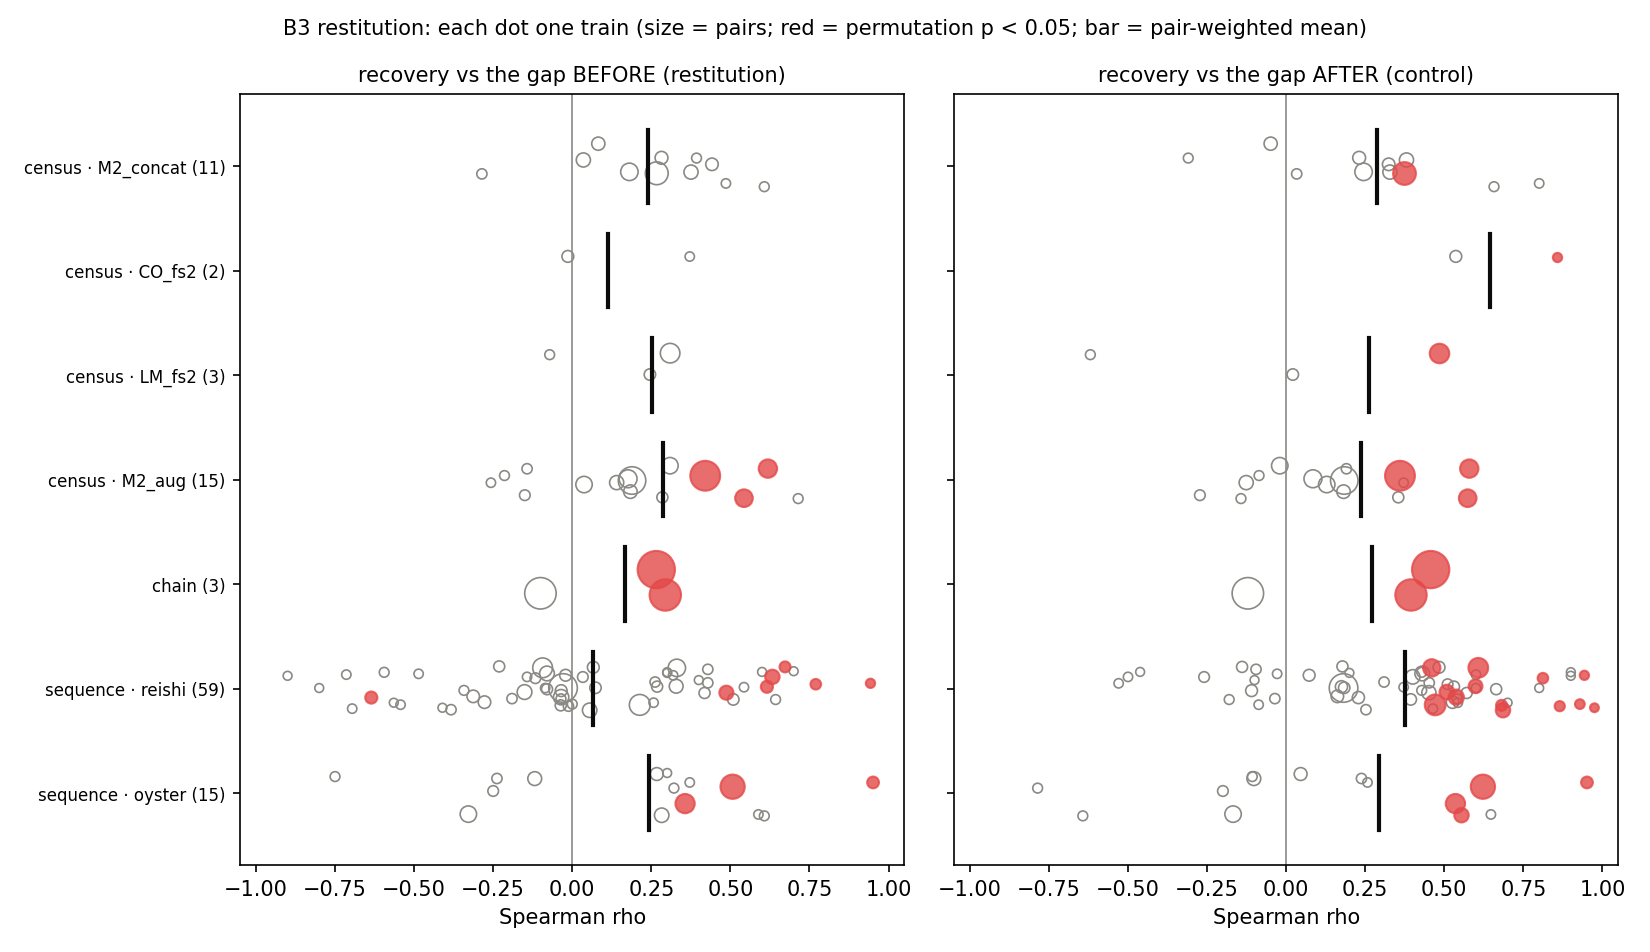
\includegraphics[width=\textwidth]{data/ch10_fhn/b3_restitution_rho.png}
\caption{Restitution. Each dot is one train's Spearman $\rho$ between recovery time and the gap before each drop (left) or the gap after it (right, a control). Dot size is the number of pairs, red marks permutation $p<0.05$, and bars are pair-weighted means. Recovery correlates as strongly with the gap after as with the gap before: a censoring artefact, not restitution.}
\label{fig:b3restitution}
\end{figure}

\section{Shapes and families across recordings}
\label{sec:rb_families}

\begin{instructions}
\textbf{B6}: do the same shape families occur across recordings and species? \textbf{Answered (3 Nov).}
Sources: \src{docs/rq_roundA_2/findings/b6-families-species-2026-11-03.md}; ledger J7;
Figure~\ref{fig:b6recurrence}.

\textbf{Method.} Read off the Recurrence page for g-11 (42 families, 804 members). Recording labels were shuffled
across members 10,000 times, keeping each family's size and each recording's count. \textbf{Re-run 5 Nov} with the
corrected labels (M2\_concat is oyster; chocolate oyster is a strain of \emph{P.\ ostreatus}), at two levels: species,
\emph{P.\ ostreatus} (M2\_aug, M2\_concat, CO) against \emph{H.\ erinaceus} (LM); and strain, oyster against
chocolate oyster against lion's mane. Script \src{scripts/thesis/species_rerun_b6_b12.py}; findings
\src{docs/rq_roundA_2/findings/b6-b12-species-rerun-2026-11-05.md}; ledger J7b.
\begin{itemize}
  \item \textbf{Shapes are shared across recordings.} 39 of 42 families span two or more recordings (14 span all four).
        The three single-recording families (F-35, F-53 and F-80) are all M2\_aug.
  \item \textbf{Across species, 28 of 42.} 28 families hold members of both species; 38 span two or more strains.
  \item \textbf{But not at random.} Shuffled labels leave 41.3 families mixed by recording ($p=0.023$) and 33.8 by
        species: real families are more species-specific than chance ($p=0.005$). A member's family says about twice
        as much about its origin as chance: mutual information 0.22 against 0.13 bits by recording, 0.08 against 0.04
        by species and 0.16 against 0.09 by strain (each $p\le0.0002$).
  \item \textbf{The yardstick.} The three \emph{P.\ ostreatus} recordings alone lean on one another as much
        (0.16 against 0.09 bits) as the strains do, so a lean by species or strain is no larger than a lean by
        recording.
  \item \textbf{Caveats.}
        \begin{itemize}
          \item Species is confounded with recording: \emph{H.\ erinaceus} is one recording in g-11 (LM, 76 of 804
                members).
          \item The members differ by source: those on CO, LM and M2\_concat are all accepted detector events, while
                M2\_aug's include seeds.
          \item Members within a burst are not independent, so read the effect size, not the $p$.
        \end{itemize}
\end{itemize}

\textbf{B12}: do spike and drop shapes and intervals differ between recordings and species? \textbf{Answered in the
backend (3 Nov).} Sources: \src{docs/rq_roundA_2/findings/b12-shapes-intervals-2026-11-03.md}; ledger J9;
Figure~\ref{fig:b12shape}.

The site cannot run this as posed. Interrogation reads only the 16 seed families, and its Review-selection and
prior-run sources are not wired. So every test ran on the core functions the pages call.

\textbf{Re-run 5 Nov} with the corrected labels (as B6), from the 3 Nov measurements; ledger J9b.
\begin{itemize}
  \item \textbf{Shape}, on the 716 accepted blind-queue events. The recordings differ beyond shuffled labels, but only a
        little:
        \begin{itemize}
          \item 11 of 15 features pass BH; 9 of 14 within duration bands; 7 of 10 on the duration residual;
          \item the normalised waveform gives $R^2=0.020$, $p=0.0005$, and the largest $\varepsilon^2$ is 0.062;
          \item duration-free measures do not separate them.
        \end{itemize}
  \item \textbf{Species is not shown beyond recording.} \emph{P.\ ostreatus} (517 events) against \emph{H.\ erinaceus}
        (199): 1 of 15 features passes BH, the share of falls (93\,\% against 85\,\%); 1 of 14 within duration bands and
        0 of 9 on the duration residual. The normalised waveform gives $R^2=0.004$, $p=0.03$, failing BH. The one
        difference is one recording: LM's events are 76\,\% falls, against 91--98\,\% on the others.
  \item \textbf{The yardstick.} Recordings of one species differ more than the species do: 7 of 15 features pass BH
        among the three \emph{P.\ ostreatus} recordings, and 7 of 15 between LM and MJu26a (CH10, 13--16), whose
        waveforms differ at $R^2=0.039$. By strain, 7 of 15 pass, as for the recordings the strains are made of.
  \item \textbf{Intervals}, on complete drop-detector v1 runs (45 channels). LV by dataset gives $p=0.057$ and CV2
        $p=0.070$; neither passes BH. By species, $p=0.09$ (LV) and 0.16 (CV2); by strain 0.24 and 0.38. The
        \emph{P.\ ostreatus} datasets differ among themselves ($p=0.047$ and 0.036). Median LV is M2\_aug 0.99, CO 1.06,
        M2\_concat 1.42, LM 0.82 and MJu26a (CH10, 13--16) 0.85.
  \item The fastest-edge rule calls 91\,\% of accepted events falls (76--98\,\% per recording).
\end{itemize}
\end{instructions}

\begin{figure}[htbp]
\centering
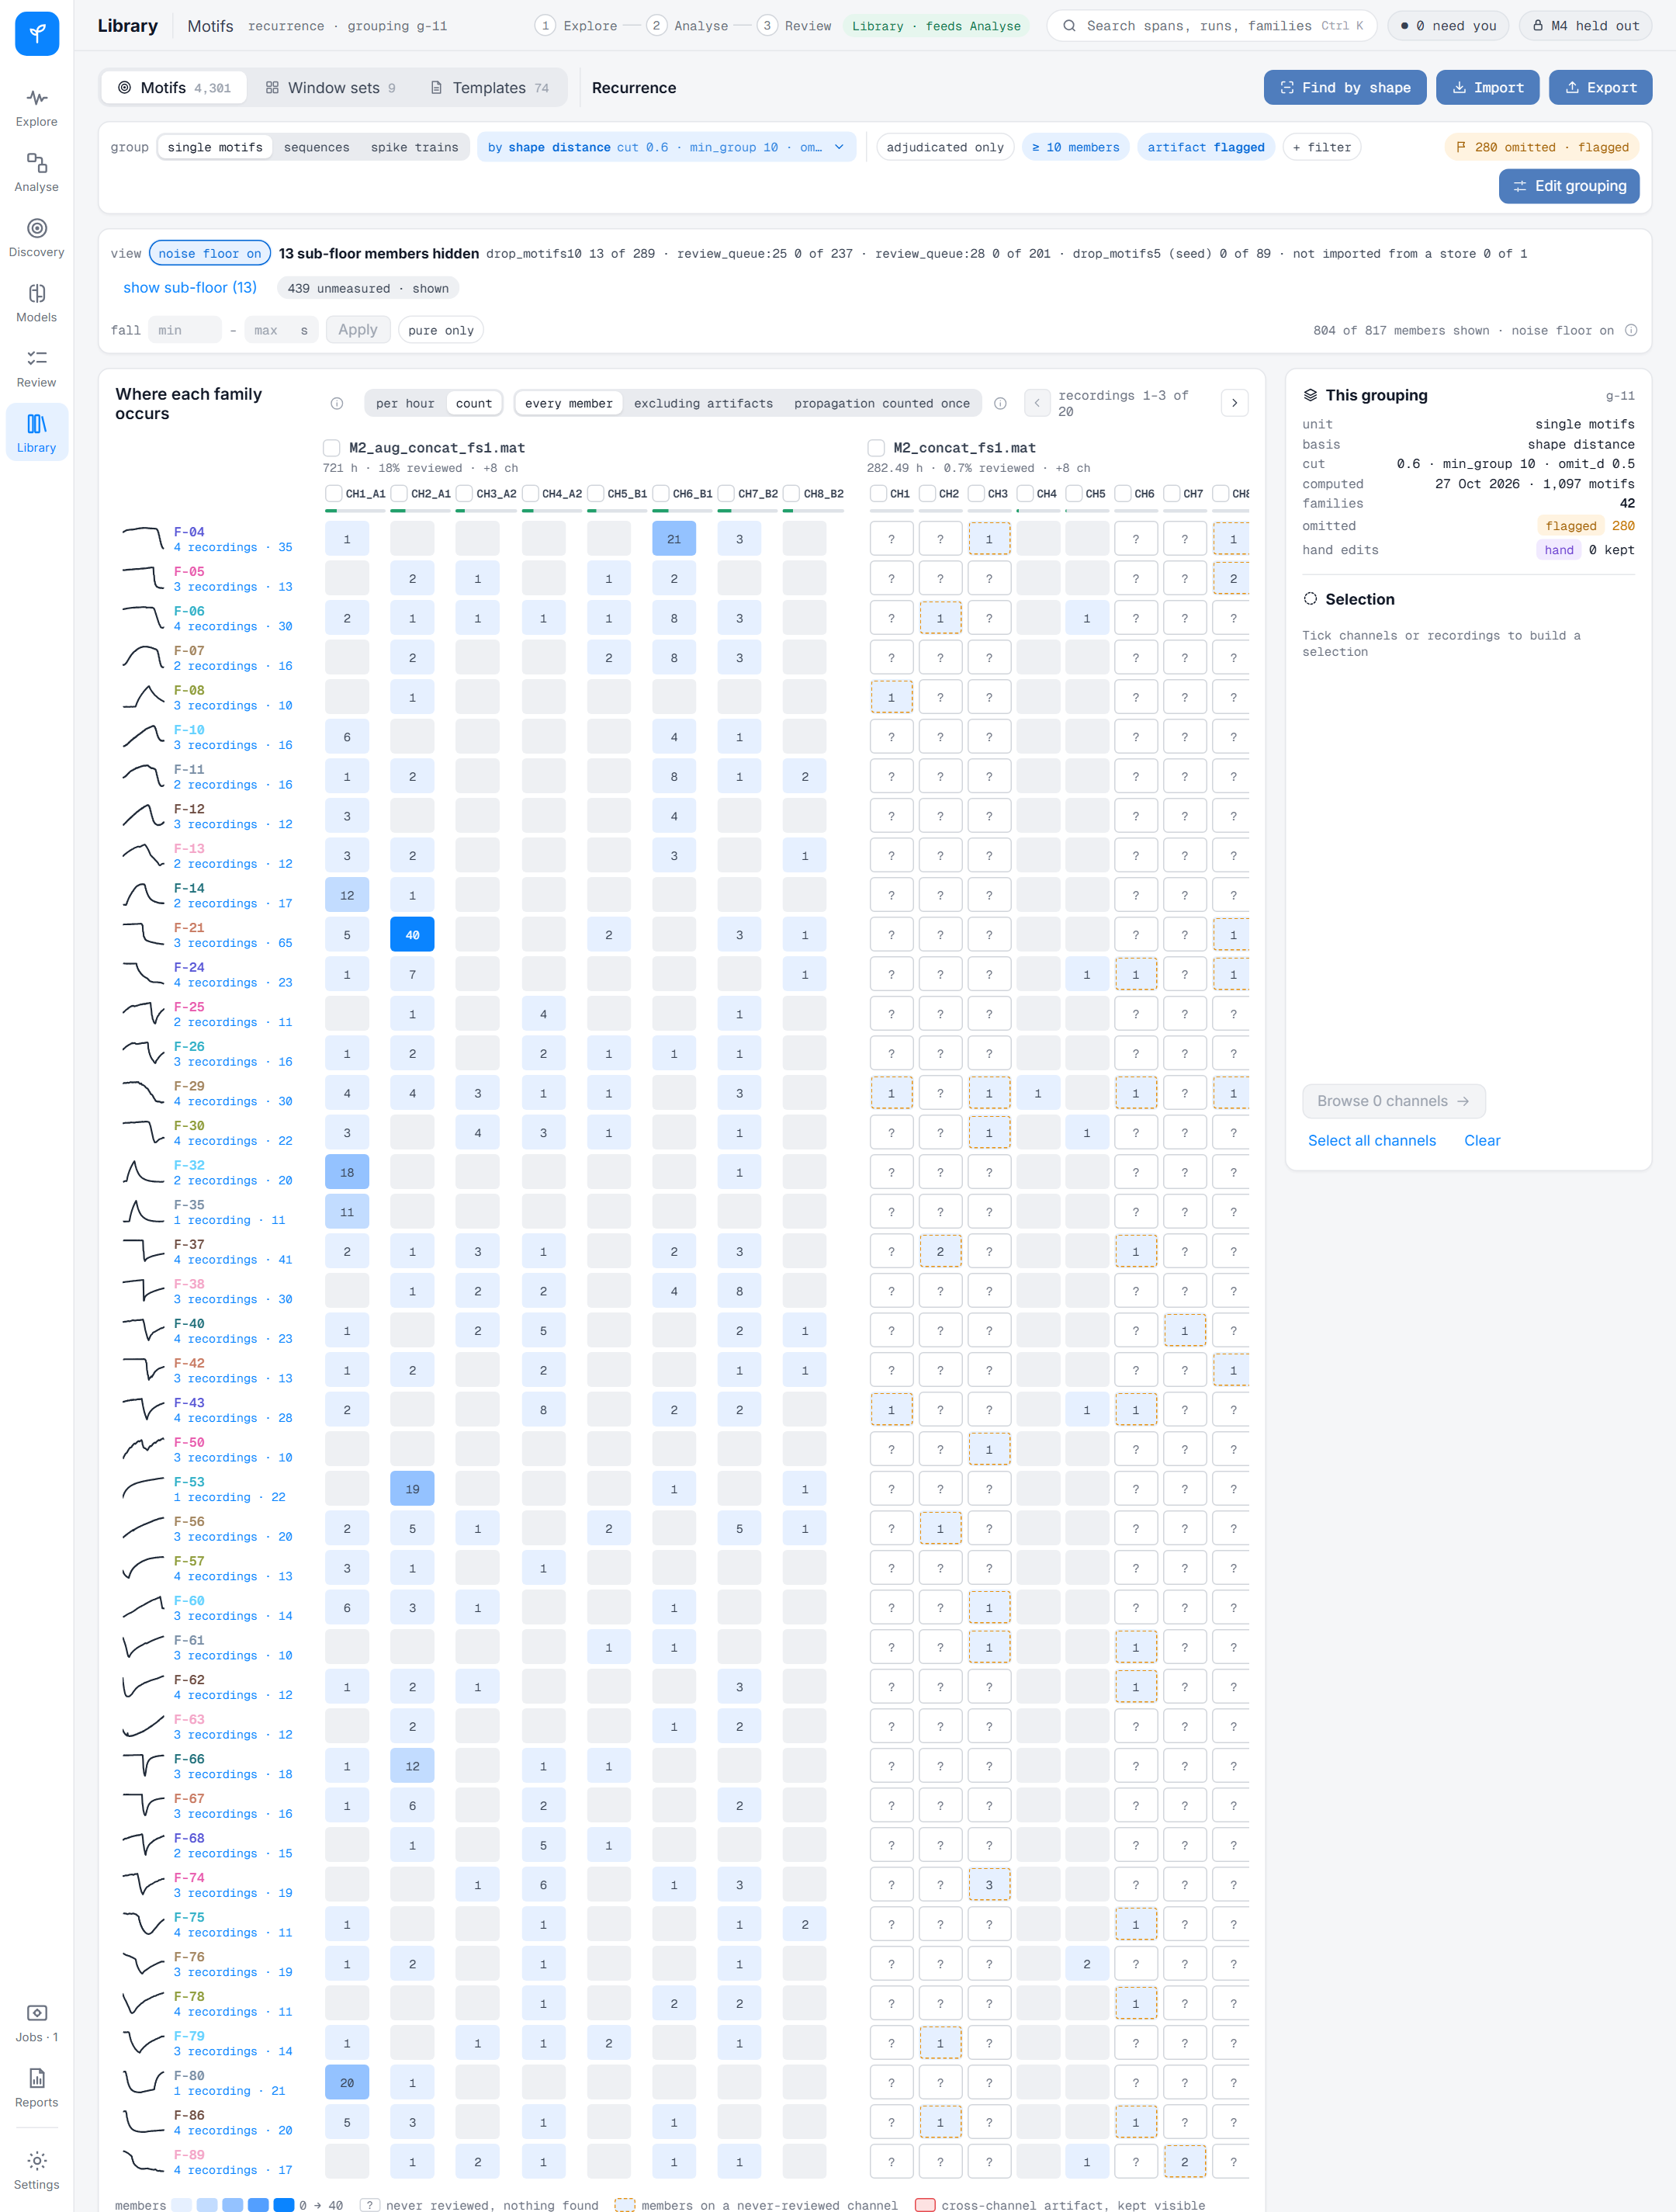
\includegraphics[width=0.72\textwidth]{roundb/b6_recurrence_g11_counts_p1.png}
\caption{B6 on the site: Library $\rightarrow$ Recurrence for grouping g-11, member counts per channel of M2\_aug, M2\_concat and CO. Each row is a family, with its shape, the number of recordings it holds and its size.}
\label{fig:b6recurrence}
\end{figure}

\begin{figure}[htbp]
\centering
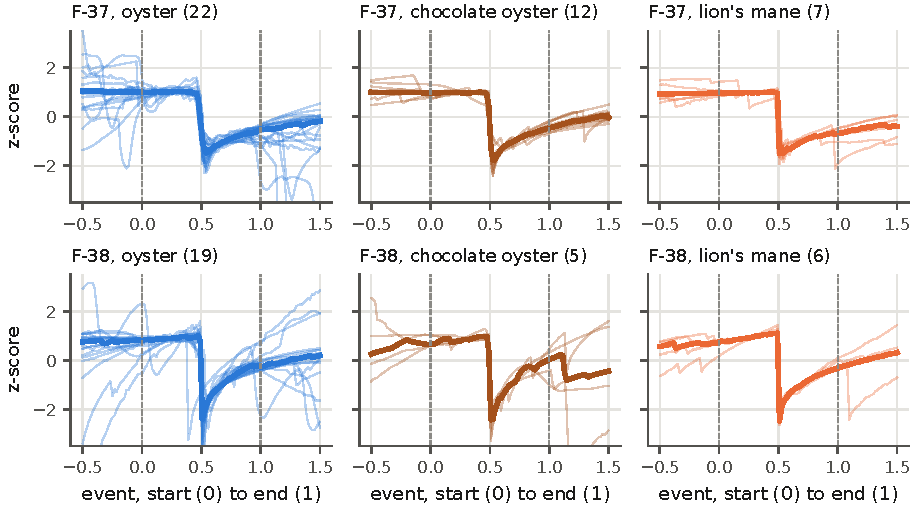
\includegraphics[width=\textwidth]{new/ch10_b6_species.pdf}
\caption{B6 in the signal: the two g-11 families with at least four members on each of the three strains, each member z-normalised and stretched so its event runs from 0 to 1 (dashed), with half its length of context either side; the bold line is the median. The same sudden fall and slow recovery appears in oyster, chocolate oyster and lion's mane.}
\label{fig:b6species}
\end{figure}

\begin{figure}[htbp]
\centering
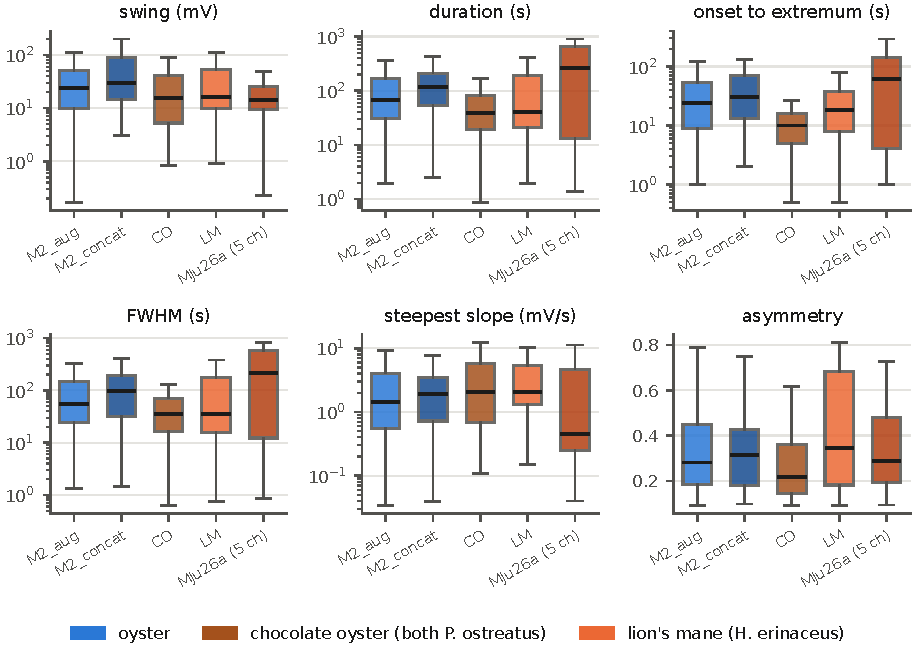
\includegraphics[width=\textwidth]{new/ch10_b12_shape.pdf}
\caption{B12: six shape measures of the 716 accepted blind-queue events, by recording, coloured by species and strain (boxes are quartiles, whiskers the 5--95\,\% range). The recordings differ, but only a little, and two recordings of one species differ about as much as the species do.}
\label{fig:b12shape}
\end{figure}

\begin{figure}[htbp]
\centering
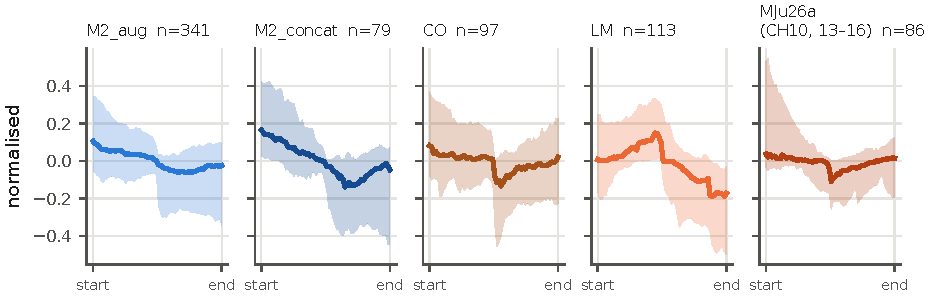
\includegraphics[width=\textwidth]{new/ch10_b12_waveforms.pdf}
\caption{B12 in the signal: each recording's accepted events stretched to a common length (start to end of the judged span), with the median shift and range removed; the line is the median and the band the middle half. Every recording's typical event is a fall, placed at different points in its span; the shapes differ in detail, and LM's events more often begin with a rise.}
\label{fig:b12waves}
\end{figure}

\section{Activity across channels}
\label{sec:rb_channels}

\begin{instructions}
\textbf{B4}: is cross-channel activity propagation, or an artefact of the shared ground? This is the plan's RQ6.
Explore $\rightarrow$ Cross-channel cannot answer it yet. The cross-channel workshop (27 Oct) specified the explorer that
will: \src{docs/rq_roundB/B4-cross-channel.md}, \src{docs/prompts/changes/cross-channel-explorer.md} (slices S0--S9)
and its decisions note, which holds a paragraph for this section. The design:
\begin{itemize}
  \item the unit is a detector census (\texttt{drop\_detection\_v1} by default), not Library members, whose selection
        reflects where people looked;
  \item M2's packs A--D are separate: propagation is judged only within a pack, a cross-pack copy is an artefact, and
        a cross-pack co-occurrence that is not a copy is a \emph{shared driver};
  \item co-occurrence means onsets within 50\,s; the bins are artefact, propagation, shared driver and independent;
  \item nulls: rotation for co-occurrence, random time for waveforms, a random-time lag pool for the timetable;
        Benjamini--Hochberg at $q=0.05$ per recording;
  \item data: the seven good datasets.
\end{itemize}
Correction: the earlier ``123 near-copy pairs, 97 beating chance, 64 flagged'' came from a sandbox copy on g-05
(4--5 Oct). The real database holds no cross-channel rows. Report B4 only if the census (S0--S1) is built and run
before the freeze; otherwise report it as designed and not run.

Built and run (28 Oct; the researcher approved S0 and S1). S0 (\src{Working/channel_layout.py}) places each channel
in a pack. S1 (\src{Working/cross_census.py}) is the census, reviewed by a critic, fixed and merged. It ran through
the site on the four recordings with a full \texttt{drop\_detection\_v1} census. The tables come from
\src{scripts/thesis/b4_cross_channel.py}, run on a backup taken after the census, into
\src{docs/thesis/data/ch10_b4/}; every census is fresh, and each carries its hash.
\begin{itemize}
  \item \textbf{M2\_aug} (packs A--D): 688 events, 26 co-occurrences. Within packs, 8 co-occurrences against a
        rotation null of 1.9 ($p=0.002$). After Benjamini--Hochberg over 24 within-pack pairs, one pair survives:
        CH15\_D2--CH16\_D2 (pack D), 2 co-occurrences against 0.01 expected. Its timetable (the delay test) finds no
        consistent lag ($L=21$\,s, $p=1.0$ on two events). \textbf{No evidence of propagation.}
  \item Across packs, 18 co-occurrences that are not copies, against a rotation null of 6.3 ($p=0.001$). Separate
        packs react together more often than chance, but this is a shared driver, never propagation. The likeliest
        candidates are a common stimulus (environment) or the electrical setup.
  \item \textbf{M2\_concat} (no packs set, one unassigned pack): 310 events and 91 co-occurrences, of which 90 are
        copies, the same waveform at the same instant. Six pairs among channels 5--8 co-occur 12--19 times each
        against fewer than 0.11 expected (all $q=0.0025$). Four electrodes moving identically at once point to the
        recording setup (a shared-ground artefact), not to the mycelium. Set M2\_concat's packs before quoting it
        further.
  \item \textbf{CO and LM}: no co-occurrence at all (37 and 125 events on four channels each); chance gives about 0.
  \item \textbf{MJu26a} (2\,Hz, 16 channels; packs not set). The census ran through the site on 5 Nov, after the
        first part of the 2\,Hz sweep was imported.
        \begin{itemize}
          \item 463 events and 16 co-occurrences, against 3.2 under rotation ($p=0.001$). Ten pairs survive
                Benjamini--Hochberg, but on one to three co-occurrences each.
          \item Seven of the 16 are copies (the same waveform at the same instant), and eight are independent
                recurrences.
          \item The two pairs with a timetable (CH1--CH2, CH1--CH6) co-occur at zero lag ($p=0.23$--0.25 against the
                lag null). The one co-occurrence with a lag (CH3--CH7, 3.5\,s) is a single event.
          \item \textbf{No evidence of propagation.} Channels fire together more often than chance, at the same
                instant. Without packs, a shared driver cannot be told from the setup.
        \end{itemize}
  \item \textbf{Not included:} SH and SO, whose \texttt{drop\_detection\_v1} runs are still on the cluster.
\end{itemize}
Caveats:
\begin{itemize}
  \item one detector, a precise but sparse one (about 43 events per channel on M2\_aug);
  \item onsets come from the steepest fall, because the real runs carry no onset label;
  \item the breadth null runs under rotation as a stated deviation from D18 (Chapter~\ref{ch:method});
  \item the bin counts in Figure~\ref{fig:b4bins} are classifications, not tests; the claims are the tests above.
\end{itemize}
\end{instructions}

\begin{figure}[htbp]
\centering
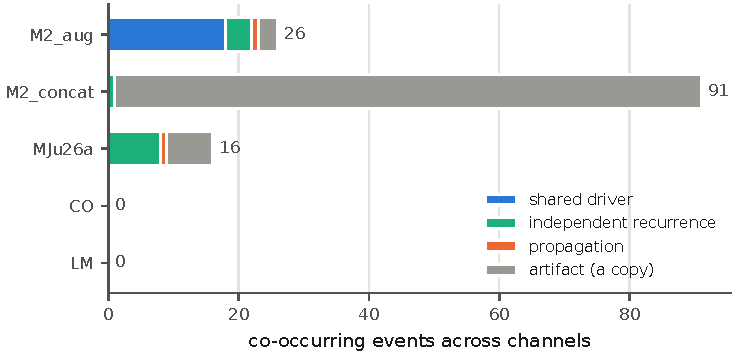
\includegraphics[width=0.85\textwidth]{new/ch10_b4_bins.pdf}
\caption{The B4 census: \texttt{drop\_detection\_v1} events that occur on two or more channels together, per recording, by what the census classifies them as. These are per-event classifications, not tests; the tests against rotation and random-time nulls are in the text. M2\_concat's are copies between channels; CO and LM have none.}
\label{fig:b4bins}
\end{figure}

\begin{figure}[htbp]
\centering
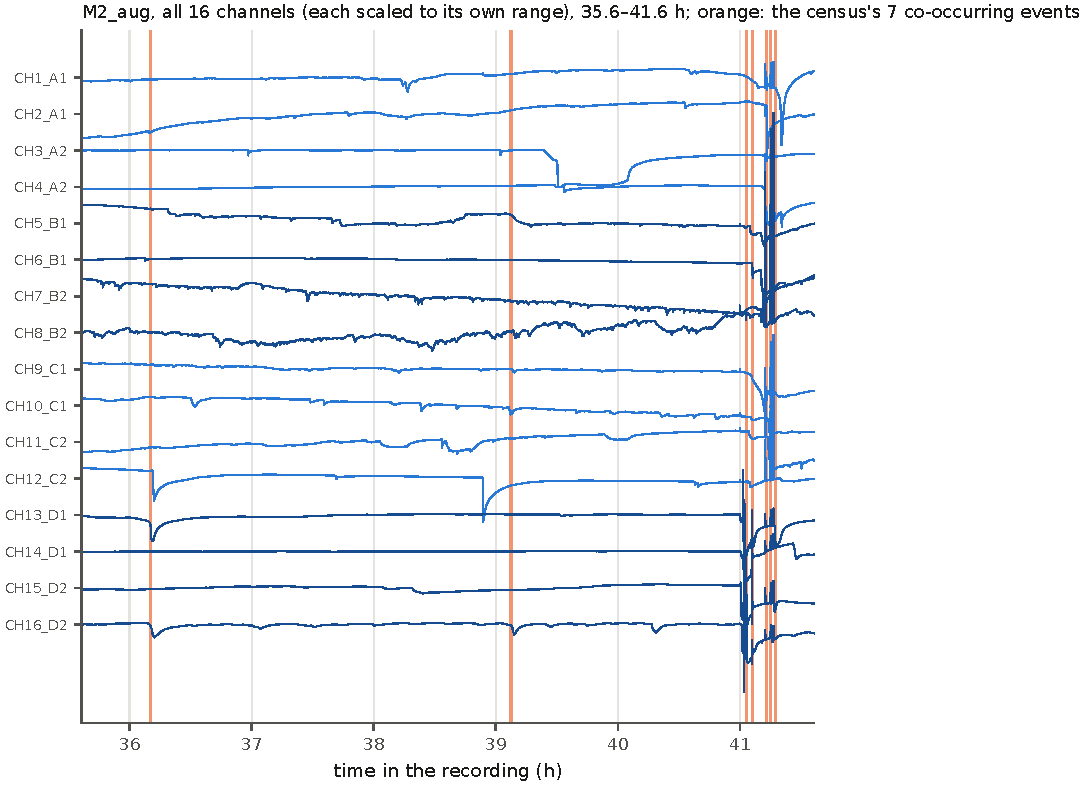
\includegraphics[width=\textwidth]{new/ch10_b4_stack.pdf}
\caption{Cross-channel co-occurrences in six hours of M2\_aug. (a) The census marked seven pairs of detections (vertical lines). Traces are scaled and clipped for the overview. The coloured markers locate the two pairs enlarged below. (b) A near-copy on CH10 and CH11, with zero waveform lag and a correlation of 0.982. (c) A candidate on CH15 and CH16 with a waveform lag of 21\,s and a correlation of 0.680. Each inset shows voltage change from the local baseline, with vertical lines at the detected onsets. The lag candidate illustrates one pair of events. The census tests found no consistent lag across events.}
\label{fig:b4stack}
\end{figure}

\section{What the detectors show}
\label{sec:rb_detectors}

\begin{instructions}
\textbf{B5}: what do the Discovery Maps show about when and where the detectors fire? \textbf{Answered (3 Nov).}
Sources: \src{docs/rq_roundA_2/findings/b5-map-timing-2026-11-03.md}; ledger J8; Figure~\ref{fig:b5timeline}.

\textbf{Method.} Read from the Map's channel level in 3-hour bins, on the five swept recordings (45 channels). The
script bins exactly as the page does: all 39 settings on M2\_aug CH6 match.
\begin{itemize}
  \item \textbf{Where.} The loose families (noise threshold, the wavelet prototype, the hour-scale CNNs) fire
        everywhere, and the drop detectors are sparse. A few channels carry far more for some families: M2\_aug CH16,
        and M2\_concat CH3 and CH8.
  \item \textbf{When.} On every channel the settings' rates rise and fall together: co-modulation 0.21--0.35 (median
        per recording), against 0.00 under random time shifts. The paired phase-randomised surrogates reach only
        0.02--0.04. So the bursts and quieter stretches are the recordings' own changes over hours and days.
  \item \textbf{Channels.} Channels rise and fall together on M2\_aug, CO and MJu26a's five-channel copy (B4's shared driver), but not on
        LM. On M2\_concat the surrogates band as well, because CH5--8 are copies.
  \item \textbf{Silence.} No 3-hour bin is ever silent: the loose detectors fire everywhere.
  \item \textbf{Caveats.}
        \begin{itemize}
          \item Detector variants share events, so co-modulation measures agreement on when, not independent
                witnesses.
          \item There is one surrogate draw per run.
          \item This cannot tell whether the changes are biological or the room's.
        \end{itemize}
\end{itemize}

\textbf{B5 on the 2\,Hz sets} (5 Nov; \src{docs/rq_roundA_2/findings/rq4n-partial-2026-11-05.md}; ledger J8b;
Figure~\ref{fig:b5newsets}). The first cluster round returned 31 of the 129 jobs whole:
\begin{itemize}
  \item 13 settings on MJu26a, and 9 each on SH and SO;
  \item the settings are OASIS, deconvolved troughs and wavelet encoded, plus, on MJu26a, \texttt{drop\_detection\_v1},
        symbol search and the wavelet prototype.
\end{itemize}
On those settings the same read gives:
\begin{itemize}
  \item \textbf{When.} Co-modulation per channel, median by recording, is MJu26a 0.33, SH 0.46 and SO 0.42, against
        0.00 under random time shifts and 0.08--0.13 for the paired surrogates. All 24 channels beat their shifts.
  \item \textbf{Channels.} Channels band together on SO (0.40, $p=0.005$; its surrogate 0.04), but not on SH (0.07,
        $p=0.24$). On MJu26a the surrogates band more than the recording (0.28 against 0.15), so its banding is not
        shown.
  \item \textbf{Caveats.} The same as above, and a stronger first one: these 9--13 settings, mostly from three
        families, share more events than the 38--44 settings on the other recordings.
\end{itemize}

\textbf{B11}: do the detectors find the same events on the newer datasets?
\begin{itemize}
  \item On the site: Discovery $\rightarrow$ Compare, and Compare every stage.
  \item Data: CO, LM and the 2\,Hz copies of MJu26a, SH and SO.
  \item Null: each run's surrogate.
  \item Needs the whole 2\,Hz sweep. Updated return audit (8 Nov): 729/1,014 tasks are complete and 79/129 settings have every channel back. A recovery bundle covers the remaining 285 tasks. The older 5 Nov map/timing results above still describe their original 31-setting subset; they have not been recomputed using the larger partial return.
  \item State the lesson of Chapter~\ref{ch:rq1}: one-draw surrogate counts measure a detector's response to the
        spectrum, not event quality.
\end{itemize}
\end{instructions}

\paragraph{Additional 2\,Hz returns.}
The returns inspected on 8 November contained 497 completed tasks on MJu26a, and 116 each on SH and SO, from planned totals of 674, 170 and 170 respectively. Complete channel coverage was available for 25, 26 and 28 settings respectively. A further 258 tasks were missing and 27 had failed, including temporary-file write conflicts and disk-I/O errors. These incomplete computations are not zero-detection results.

On settings with complete coverage, OASIS and the drop detector returned more detections in the recordings than in their paired phase-randomised copies, while the wavelet-encoded setting returned substantially more in the surrogates (Table~\ref{tab:rq4partialreturns}). This reproduces the distinction between detectors responding differently to phase scrambling. One draw per channel gives a count comparison, not a well-resolved null distribution, and neither direction establishes human acceptance. The outstanding CNN and matrix-profile tasks prevent a complete comparison of agreement across all detector families.

\begin{table}[htbp]
\centering
\caption{Selected settings with every planned channel returned in the 2\,Hz extension. Cells give real/surrogate detection counts, summed over 16 channels for MJu26a and four each for SH and SO. Each channel has one phase-randomised surrogate. These are detection counts, not grouped or human-accepted event counts.}
\label{tab:rq4partialreturns}
\small
\begin{tabularx}{\textwidth}{@{}Xrrr@{}}
\toprule
\textbf{Setting} & \textbf{MJu26a} & \textbf{SH} & \textbf{SO}\\
\midrule
Drop v1 & 463/33 & 21/0 & 28/0\\
OASIS, default & 127,429/2,007 & 20,095/353 & 25,556/364\\
OASIS, threshold 5 & 2,453/68 & 859/19 & 400/11\\
Wavelet encoded, default & 1,883/38,714 & 21/7,241 & 12/7,286\\
\bottomrule
\end{tabularx}
\end{table}

% Additional return counts: data/hpc_return_20261108/rq4_summary.csv and audit.json.
% No new human verdicts or completed B11 agreement analysis are claimed here.

\begin{figure}[htbp]
\centering
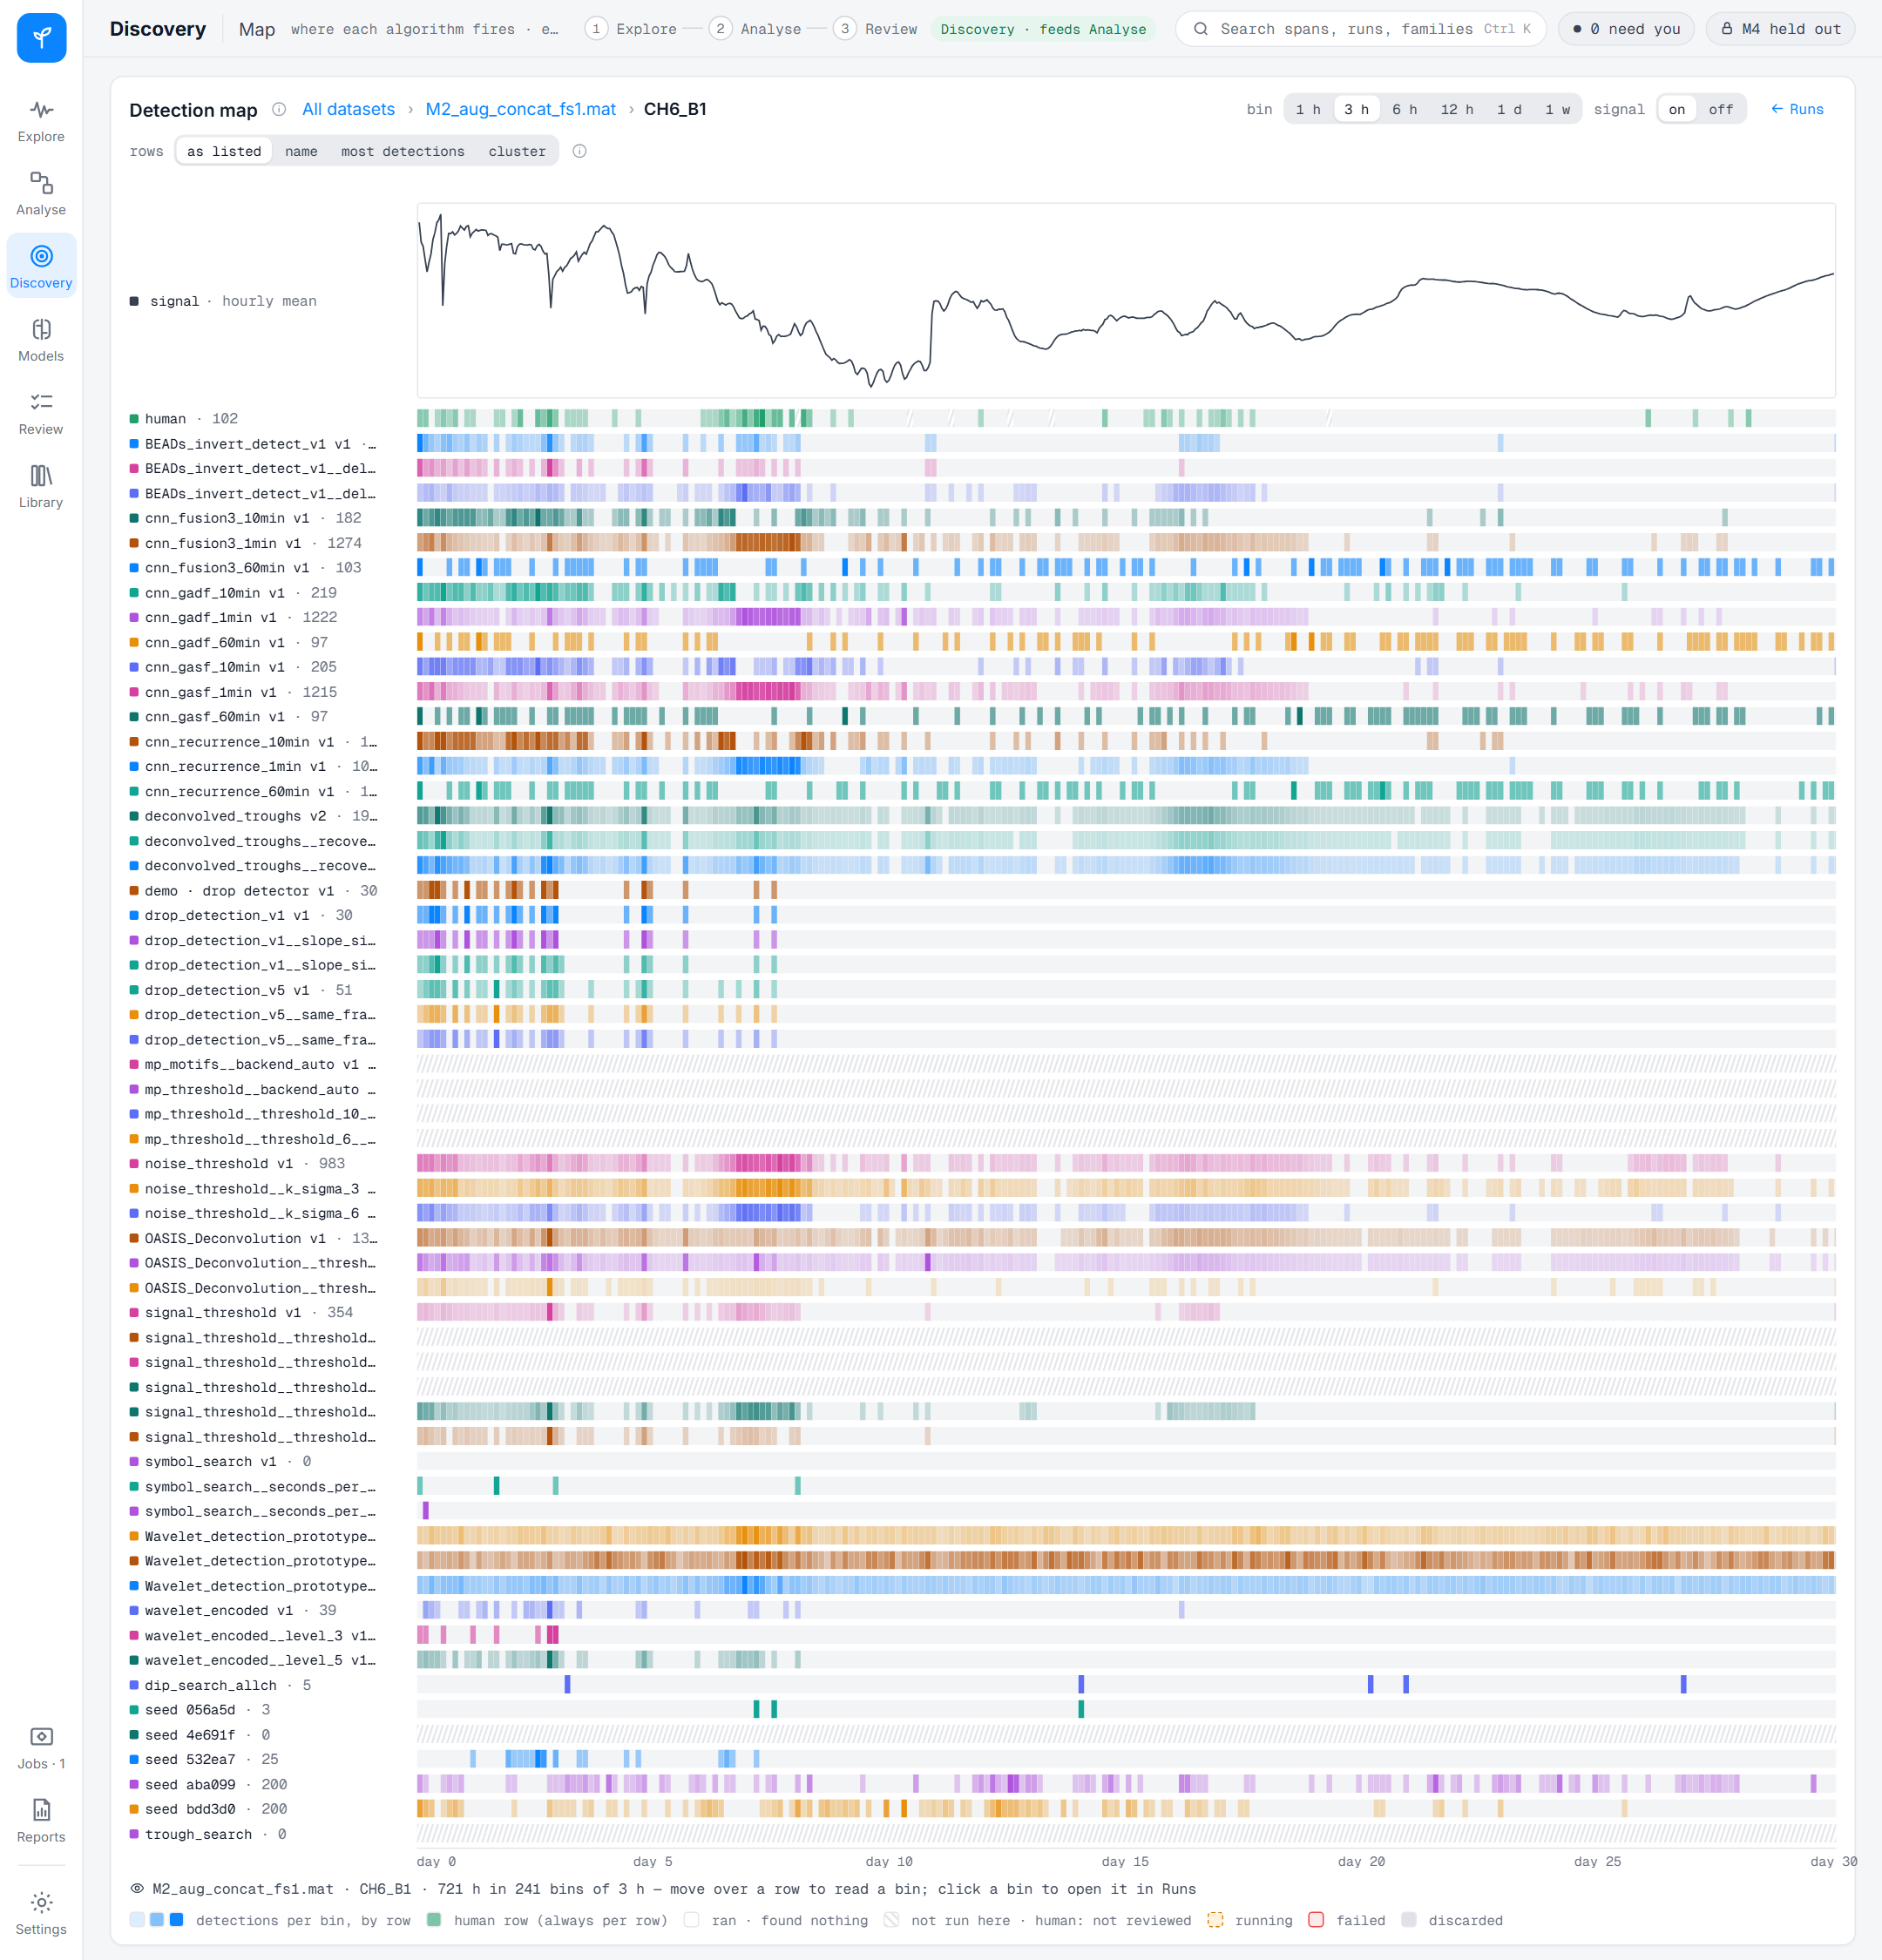
\includegraphics[width=0.85\textwidth]{roundb/b5_map_channel_M2_aug_CH6.png}
\caption{B5 on the site: Discovery $\rightarrow$ Map, M2\_aug CH6. Every detector setting is shown in 3-hour bins over 30 days, under the signal's hourly mean. Most settings fire densely in days 0--8 and around days 15--17 and thin out together elsewhere. This is the co-modulation that the paired surrogates do not reproduce.}
\label{fig:b5timeline}
\end{figure}

\begin{figure}[htbp]
\centering
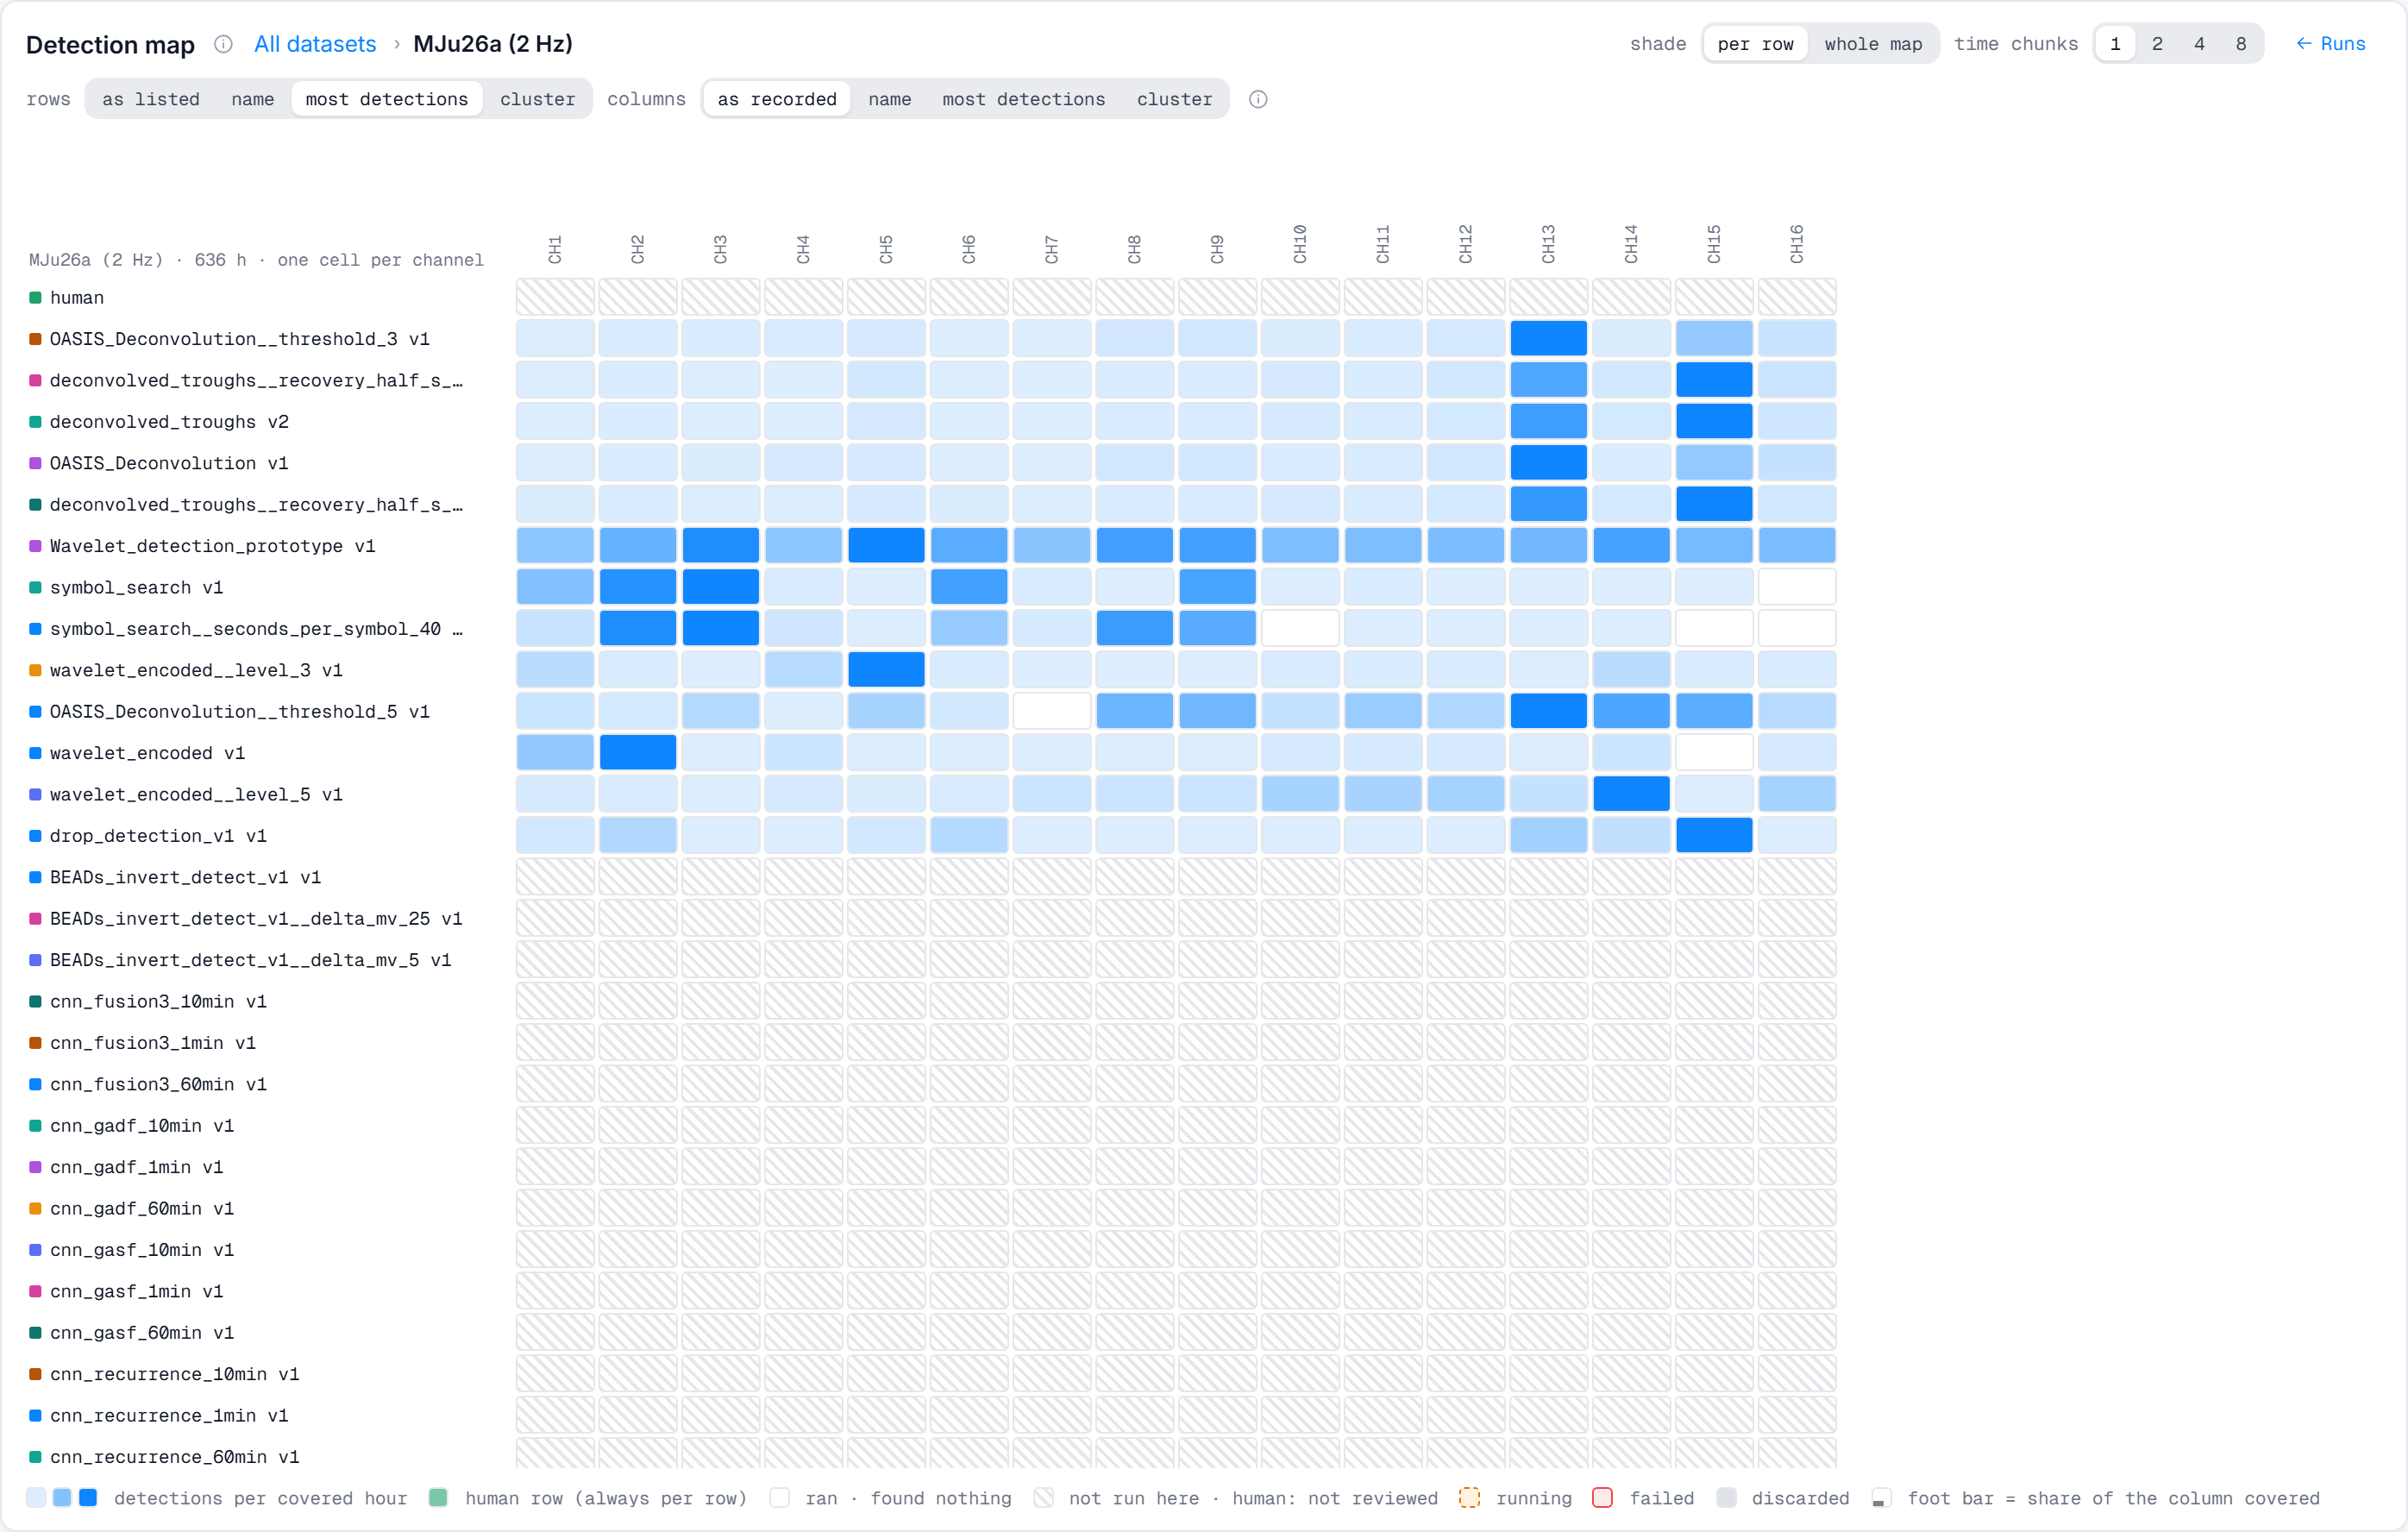
\includegraphics[width=0.85\textwidth]{roundb/b5_map_dataset_MJu26a_fs2.png}
\caption{The first part of the 2\,Hz sweep on the site: Discovery $\rightarrow$ Map, MJu26a (2\,Hz), one cell per channel and setting, with rows sorted by detections. The 13 settings whose jobs came back whole are filled; the rest (hatched) still have to run on the cluster.}
\label{fig:b5newsets}
\end{figure}

\section{Time scales and methods from other fields}
\label{sec:rb_methods}

\begin{instructions}
Each study asks what a method borrowed from another field reveals on fungal signals, and whether it beats its null.
\begin{itemize}
  \item \textbf{B9}, CWT ridges (mass spectrometry), on the \texttt{cwt\_events} template. Is event duration
        multimodal, as Adamatzky's three scales suggest? \textbf{Answered, negative (3 Nov).}
        Sources: \src{docs/rq_roundA_2/findings/b9-cwt-durations-2026-11-03.md}; ledger J10; Figure~\ref{fig:b9hist}.
        \begin{itemize}
          \item \textbf{Data.} 20 one-day spans (4 channels $\times$ 5 recordings), each with one AAFT and one
                phase-randomised copy.
          \item \textbf{Counts.} The real recordings give 632 drops (260 clean). Their AAFT copies give 1,087 (517).
                Only 6 of 20 spans beat their copy, and no recording does overall.
          \item \textbf{Durations.} The same single skewed pile, from about 15\,s to minutes: KS $p=0.39$--0.83 per
                recording, pooled 0.59. The one exception is M2\_concat, longer ($p=0.007$).
          \item \textbf{Modes.} A mixture fit finds ``modes'' at 17\,s and 87\,s, and finds them more strongly in
                AAFT. So they are the detector reading noise of this value distribution, not preferred event scales.
          \item \textbf{On the site.} Analyse agrees on M2\_aug: real 93, AAFT 51, phase 0.
          \item \textbf{Consequence.} W1's ``beats its null'' held only against the phase null, which turns the
                lopsided value distribution into a bell curve and then yields almost no drops. Against AAFT,
                \texttt{cwt\_events} does not find structure beyond its input's values. Re-judge it before citing it.
        \end{itemize}
  \item \textbf{B10}, structure across scales. \textbf{Answered (3 Nov).}
        Sources: \src{docs/rq_roundA_2/findings/b10-scales-2026-11-03.md}; ledger J11; Figure~\ref{fig:b10motif}.
        \begin{itemize}
          \item \textbf{Matrix profile on the site.} \texttt{motif\_lengths} ran on one 8\,h span per recording
                (channel 0, from the middle). The lengths that repeat beyond AAFT are:
                \begin{itemize}
                  \item M2\_aug 30\,s--16.3\,min, M2\_concat 30\,s--4.4\,min, CO 30\,s--25.1\,min and LM
                        30\,s--16.3\,min;
                  \item none on MJu26a, whose span is a steady oscillation of about 20\,min that AAFT keeps.
                \end{itemize}
                As in W3, the cleared lengths form one band and the strongest gap is at the shortest length, so no
                window is preferred. The 38.8\,min and 1\,h rungs cannot be judged on 8\,h.
          \item \textbf{CNN templates} (existing sweep, real against one phase-randomised copy): the 10-minute
                templates beat their copy on all five recordings and the 60-minute ones on CO, M2\_aug and MJu26a.
                The 1-minute ones beat it on none (their copies give 2--8 times more). After B9, read these margins as
                an upper bound against AAFT.
          \item Earlier result: on the MJu26a CH14 excerpt (4\,h) every judged length from 30\,s to 16\,min repeated beyond noise,
                strongest at 30\,s. \texttt{spike\_event\_features} was not run.
        \end{itemize}
\end{itemize}
State the general finding as the chapter's conclusion: which borrowed methods transfer, and which only measure the
spectrum. Include B1's interval statistics and B3's restitution test. B9 and B10 add a sharper version: the matrix profile finds
structure beyond AAFT at every judged length from 30\,s to minutes on four recordings, while \texttt{cwt\_events} does
not beat AAFT at all. The null's choice decides the verdict, as Chapter~\ref{ch:rq1} found for the detectors.
\end{instructions}

\begin{figure}[htbp]
\centering
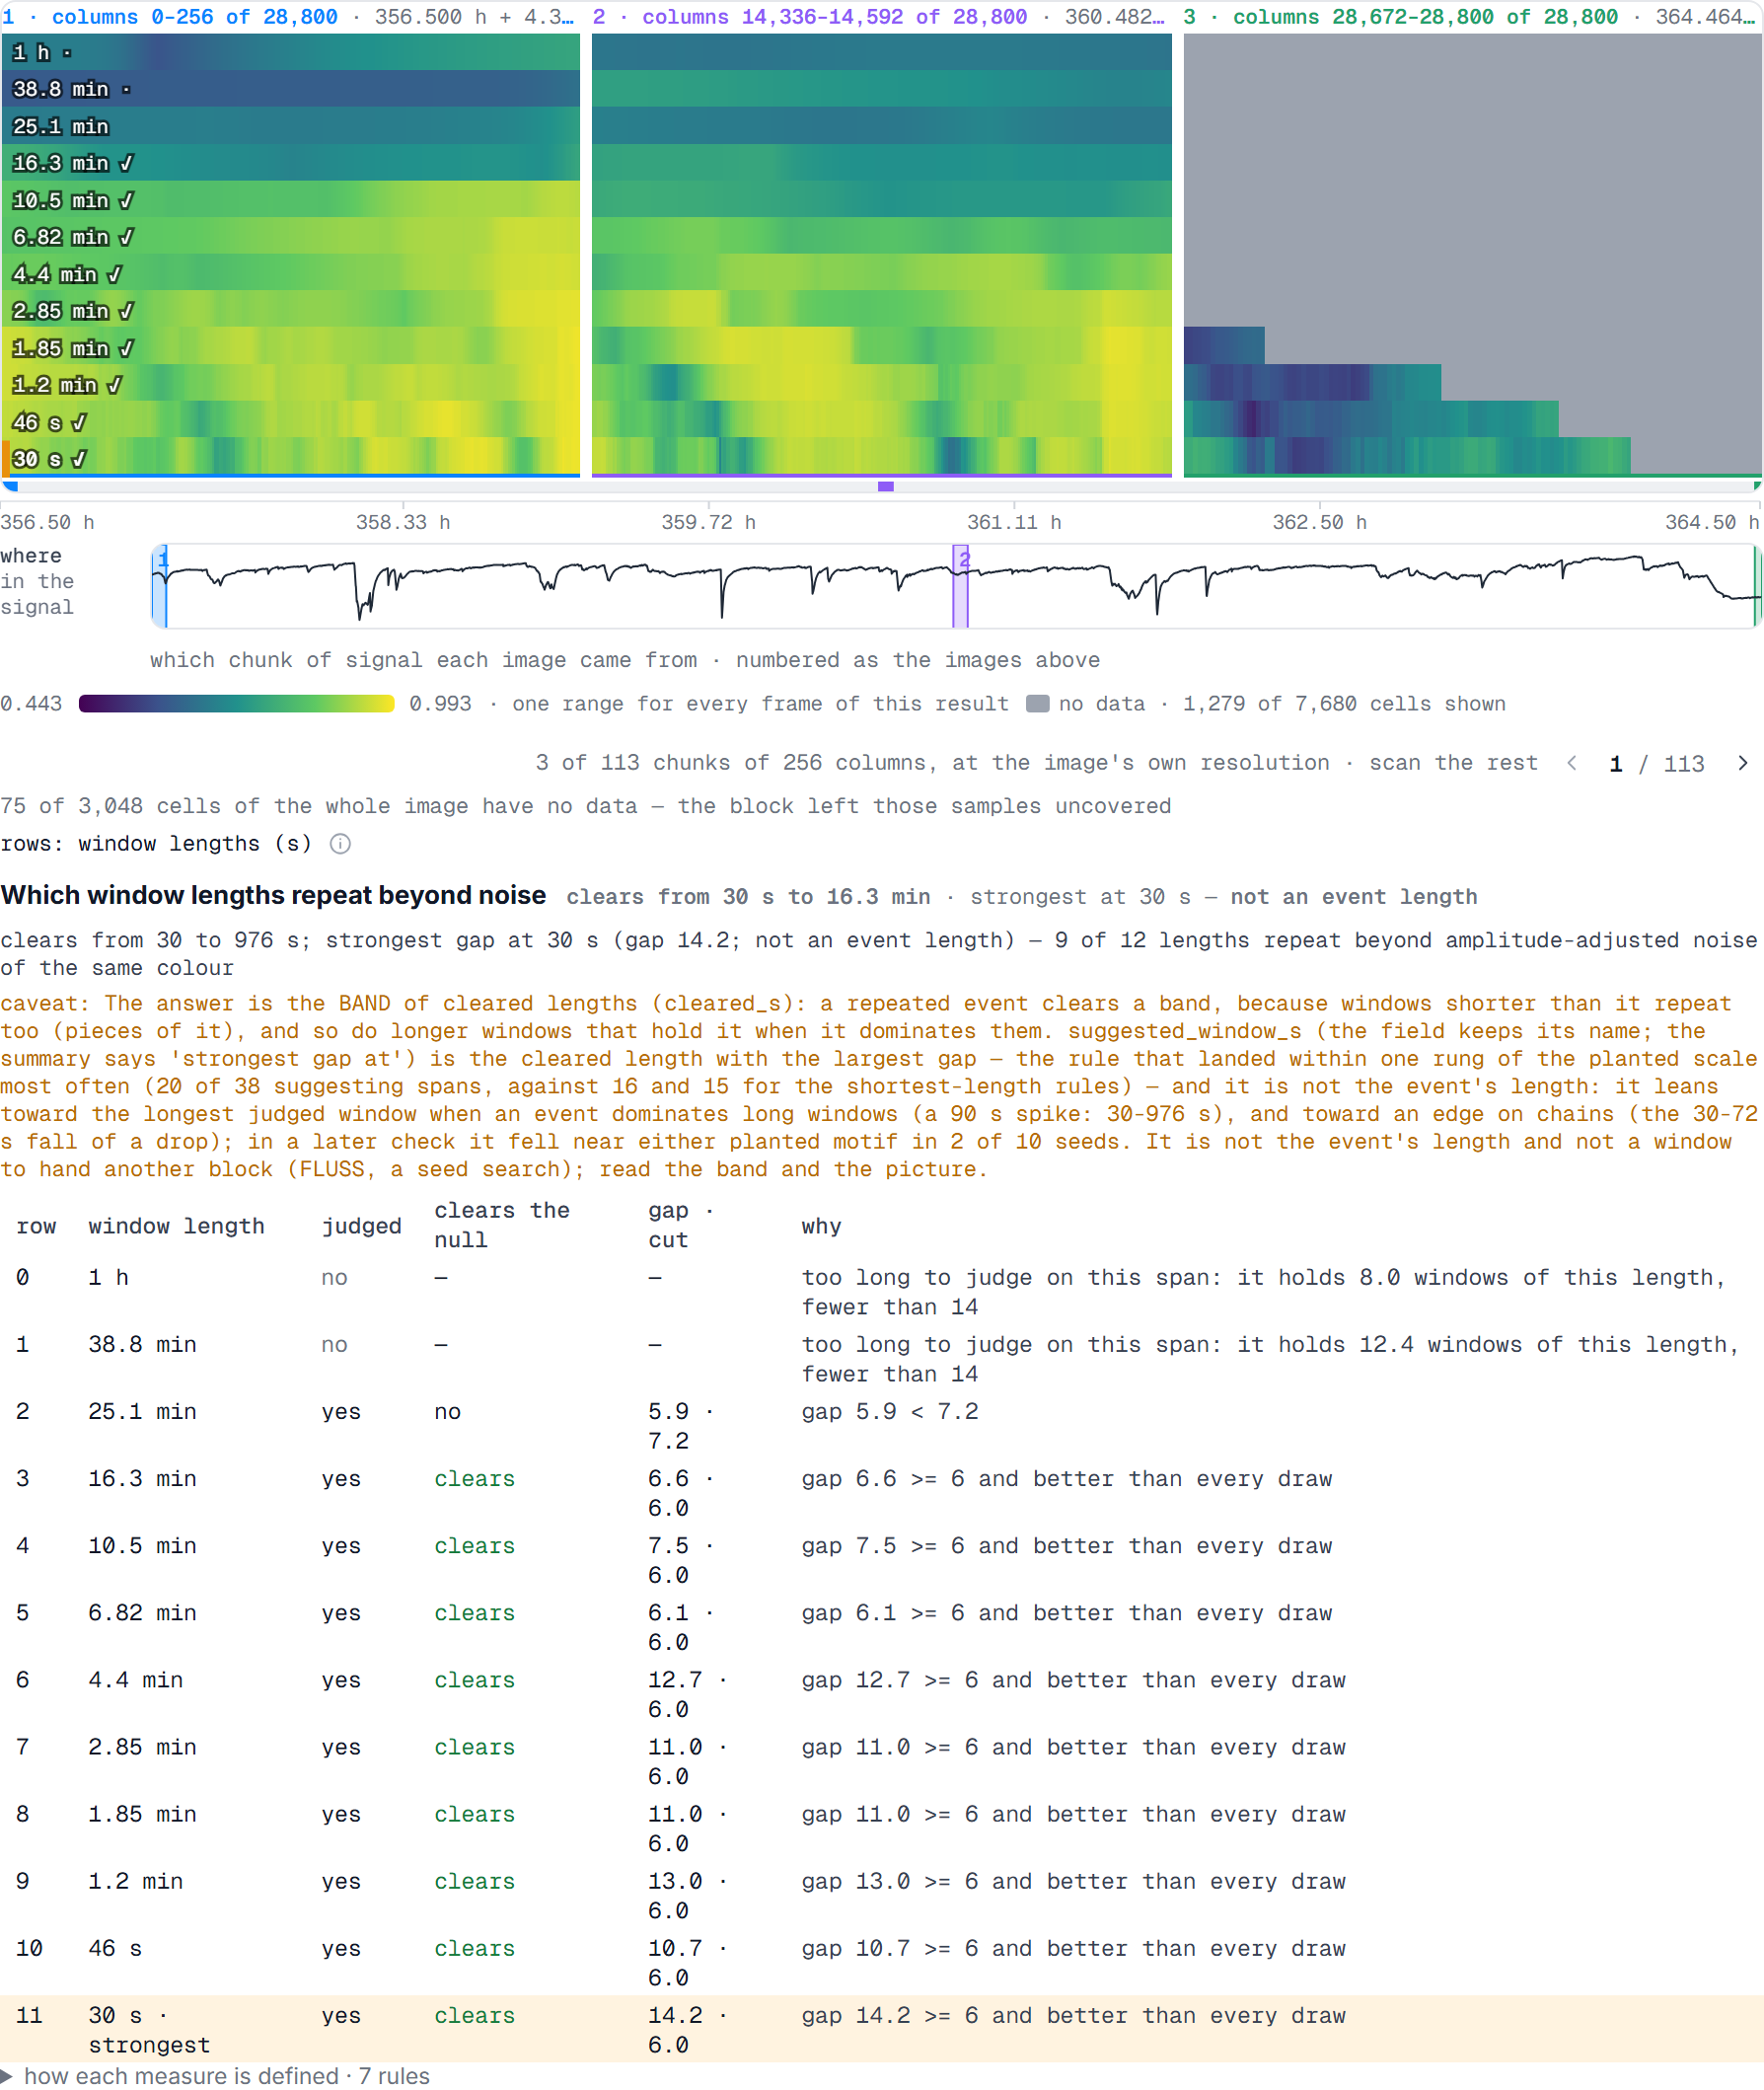
\includegraphics[width=0.78\textwidth]{roundb/b10_motif_lengths_m2aug.png}
\caption{B10 on the site: \texttt{motif\_lengths} on M2\_aug, 356.5--364.5\,h, with the pan matrix profile, the span and the verdict per window length. The lengths that repeat beyond AAFT noise run from 30\,s to 16.3\,min.}
\label{fig:b10motif}
\end{figure}

\begin{figure}[htbp]
\centering
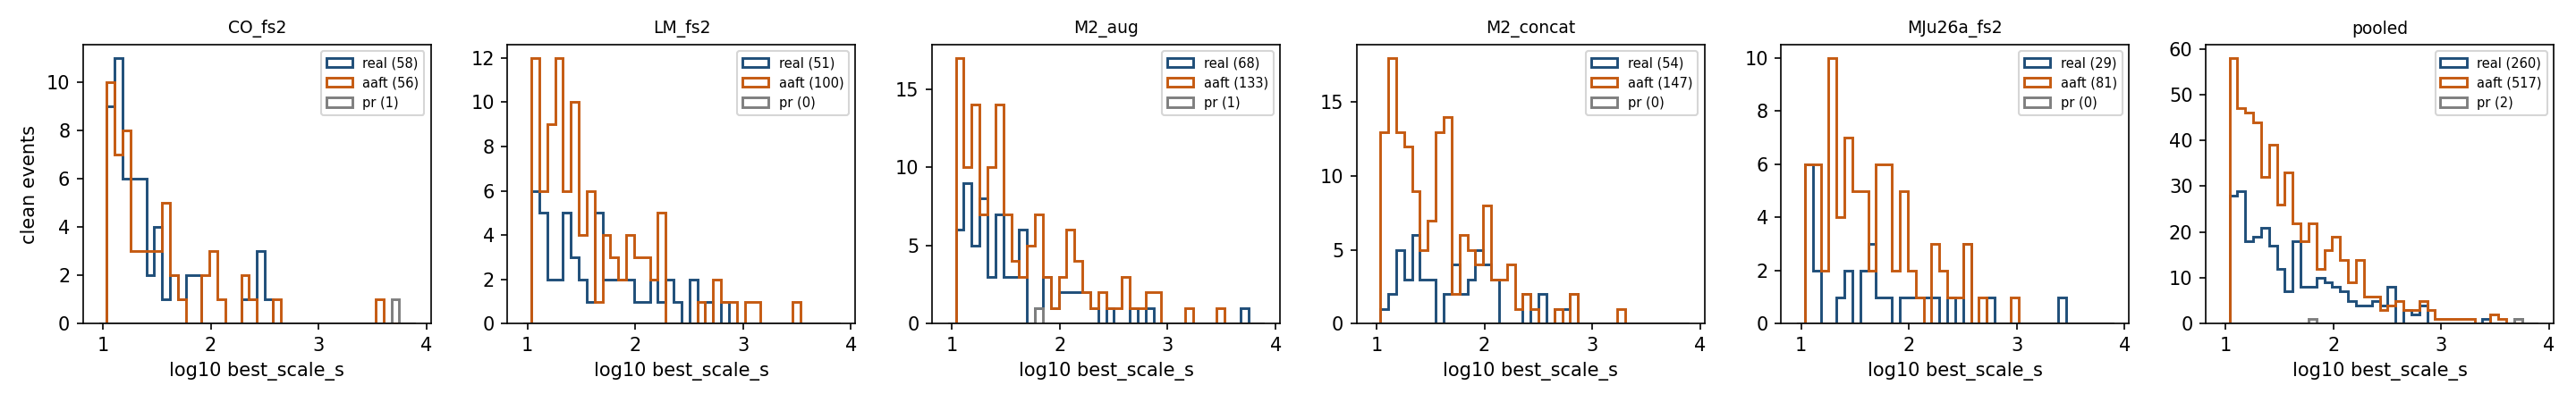
\includegraphics[width=\textwidth]{data/ch10_b9/durations_hist.png}
\caption{B9: \texttt{cwt\_events} durations (log$_{10}$ seconds), real (blue) against AAFT copies (orange) and phase-randomised copies (grey), per recording and pooled. AAFT gives more drops than the real recordings, with the same durations.}
\label{fig:b9hist}
\end{figure}

\section{Summary}

\begin{instructions}
Table~\ref{tab:rbsummary} holds every round-B result as it stood at the freeze (3 Nov); each row's number is in the
ledger (J1--J3, J6--J11; B1's final read is J1b, 5 Nov).
\begin{itemize}
  \item \textbf{Prose:} add one sentence per study on what it changes.
  \item \textbf{When the open row returns,} update it: B11 needs the 2\,Hz sweep.
  \item \textbf{B6 and B12 rows} were re-run on 5 Nov with M2\_concat as oyster and chocolate oyster as a strain of \emph{P.\ ostreatus} (ledger J7b, J9b).
  \item \textbf{Verdicts:} supported, bounded (a real but limited or partial result), not supported, or open.
\end{itemize}
\end{instructions}

\begin{table}[htbp]
\caption{The studies of this chapter at the freeze: each question's null, its result and the verdict. B3 reports only its restitution half; B7 and B8 were not run (future work), and B11 waits on the rest of the 2\,Hz sweep.}
\label{tab:rbsummary}
\fontsize{10}{11.5}\selectfont
\setlength{\tabcolsep}{4pt}
\begin{tabularx}{\textwidth}{@{}l >{\raggedright\arraybackslash}X >{\raggedright\arraybackslash}p{2.2cm} >{\raggedright\arraybackslash}p{5.4cm} >{\raggedright\arraybackslash}p{2.2cm}@{}}
\toprule
\textbf{\#} & \textbf{Question} & \textbf{Null} & \textbf{Result} & \textbf{Verdict}\\
\midrule
B1 & Are intervals regular, bursty or random? & rate-matched Poisson; shuffled intervals & 44 measurable channels, five recordings: no channel's LV leaves the Poisson band after BH (CV2: two more regular); neighbouring gaps more alike than shuffled on 18, on every recording; one alternates & supported: random-like timing with a drifting rate\\
B2 & Do sequences change shape step by step? & shuffled order & morph fraction: 0 of 5 testable sequences; step size: 5 of 19 closer than shuffled (4 after BH), ratios 0.58--0.84; 5 alternate & bounded: persistence, not a steady morph\\
B3 & Does recovery depend on the gap before it? & gaps shuffled within trains & within trains, $z=+2.9$ falls to $+0.6$ given depth, and the gap after gives $+9.9$ (censoring); across census gaps, M2\_aug $z=+5.0$ and M2\_concat $+3.1$, halved by fall duration & not within trains; bounded across census gaps\\
B4 & Propagation, or a shared ground? & rotation; random time & M2\_aug within packs 8 against 1.9 ($p=0.002$), one pair after BH, no consistent lag; across packs 18 against 6.3 ($p=0.001$); M2\_concat CH5--8 are copies; none on CO, LM; MJu26a 16 against 3.2 ($p=0.001$), both timetables at zero lag & propagation not supported; a shared driver\\
B5 & When and where do detectors fire? & random time shifts; paired surrogates & settings rise and fall together on 45 of 45 channels: 0.21--0.35 against 0.00 shifted and 0.02--0.04 for surrogates; on the 2\,Hz sets' first 9--13 settings, 24 of 24 (0.33--0.46) & supported: changes over hours to days\\
B6 & Do families recur across recordings and species? & shuffled recording labels & 39 of 42 families on two or more recordings, 28 on both species; the mix is not random (0.22 against 0.13 bits by recording, $p=0.0001$), and the lean by species is no larger than by recording & supported, with leanings by recording\\
B9 & Do event durations prefer some scales? & AAFT & AAFT copies give more drops (1,087 against 632) with the same durations (pooled KS $p=0.59$); the ``modes'' appear in AAFT too & not supported\\
B10 & At which time scales is there structure? & AAFT & every judged length from 30\,s up to 4.4--25.1\,min repeats beyond AAFT on four recordings, strongest at 30\,s; none on MJu26a & supported: one band, no preferred scale\\
B11 & Same events on the newer datasets? & per-run surrogate & 31 of the 2\,Hz sweep's 129 jobs imported; the rest back on the cluster & open\\
B12 & Do shapes and intervals differ by recording and species? & shuffled labels & recordings differ a little (11 of 15 features pass BH; $\varepsilon^2\le0.06$); species: 1 of 15 (share of falls, carried by LM), against 7 of 15 between recordings of one species; intervals borderline by dataset ($p=0.06$--0.07), not by species ($p=0.09$) & bounded: small recording effects; species not shown beyond recording\\
\bottomrule
\end{tabularx}
\end{table}
